\begin{questions}
    \ifnum \Set=1
        \ifnum \Version=1
\question[1] Give an example of a second order constant coefficient homogeneous DE whose solution is $y = c_1e^{-3t} + c_2e^{-4t}$. \vspace{2cm}
\fi 

\ifnum \Version=2
\question[1] Give an example of a second order constant coefficient homogeneous DE whose solution is $y = c_1e^{-t} + c_2e^{-2t}$. \vspace{2cm}
\fi

\ifnum \Version=3
\question[1] Give an example of a second order constant coefficient homogeneous DE whose solution is $y = c_1e^{t} + c_2e^{-2t}$. \vspace{2cm}
\fi 

\ifnum \Version=4
\question[1] Give an example of a second order constant coefficient homogeneous DE whose solution is $y = c_1e^{2t} + c_2e^{-3t}$. \vspace{2cm}
\fi 

\ifnum \Version=5
\question[1] Give an example of a second order constant coefficient homogeneous DE whose solution is $y = c_1e^{3t} + c_2e^{-5t}$. \vspace{2cm}
\fi 




\ifnum \Version > 5
\question[6] Use the method of reduction of order to determine a second solution, $y_2$, to the DE so that $\{y_1,y_2\}$ forms a fundamental set.
$$t^2y'' + ty' - y = 0, \quad t > 0, \quad y_1 = t$$
\ifnum \Solutions=1 {\color{DarkBlue} 
\textbf{Solutions:}

To use the reduction of order method, we assume a solution of the form \( y = v(t) t \), where \( v(t) \) is a function to be determined. Compute the first and second derivatives of \( y \) and substitute into DE. 
   \[ y = v(t) t \]
   \[ y' = v'(t) t + v(t) \]
   \[ y'' = v''(t) t + 2 v'(t) \]
   \[ t^2 (v''(t) t + 2 v'(t)) + t (v'(t) t + v(t)) - v(t) t = 0 \]

Simplify:
   \[ t^3 v''(t) + 2 t^2 v'(t) + t^2 v'(t) + t v(t) - t v(t) = 0 \]
   \[ t^3 v''(t) + 3 t^2 v'(t) = 0 \]
   \[ t^2 (t v''(t) + 3 v'(t)) = 0 \]

For \( t > 0 \), divide through by \( t^2 \):
   \[ t v''(t) + 3 v'(t) = 0 \]
   \[ v''(t) + \frac{3}{t} v'(t) = 0 \]

This is a first-order linear differential equation in \( v'(t) \). Let \( u = v'(t) \), so \( u' = v''(t) \):
   \[ u' + \frac{3}{t} u = 0 \]

This is a first-order linear differential equation. To solve it, we find the integrating factor:
   \[ \mu(t) = e^{\int \frac{3}{t} dt} = e^{3 \ln t} = t^3 \]

Multiply both sides of the equation by the integrating factor:
   \[ t^3 u' + 3 t^2 u = 0 \]
   \[ \frac{d}{dt} (t^3 u) = 0 \]
   \[ t^3 u = C \]
   \[ u = \frac{C}{t^3} \]
   \[ v'(t) = \frac{C}{t^3} \]
   \[ v(t) = \int \frac{C}{t^3} dt = -\frac{C}{2t^2} + C_1 \]

Now, substituting back \( y_2 = v(t) t \):
   \[ y_2 = \left( -\frac{C}{2t^2} + C_1 \right) t = -\frac{C}{2t} + C_1 t \]
   The above is sufficient, but can also write this as $y_2 = t^{-1}$. 



} 
\else 
\newpage
\fi
\fi 










        \ifnum \Version=1   
\question[4] You do not need to show your work for this question. Consider the differential equation below.
$$\displaystyle t^2 \, \frac{dy}{dt} + y = \cos(t)$$    
\begin{parts}
    \part Fill in the appropriate circle to indicate whether the DE is linear or non-linear
    \begin{itemize}
        \item[$\bigcirc$] The DE is linear.
        \item[$\bigcirc$] The DE is non-linear.
    \end{itemize}
    \part Indicate whether the DE is autonomous or non-autonomous. 
    \begin{itemize}        
        \item[$\bigcirc$] The DE is autonomous.
        \item[$\bigcirc$] The DE is non-autonomous.
    \end{itemize}    
    \part Indicate whether the DE is homogeneous or non-homogeneous. 
    \begin{itemize}        
        \item[$\bigcirc$] The DE is homogeneous.
        \item[$\bigcirc$] The DE is non-homogeneous.
    \end{itemize}    
    \part What is the order of the DE? \framebox{\strut\hspace{4cm}}
    \vspace{12pt}   
    
\end{parts}
\ifnum \Solutions=1 {\color{DarkGreen} 
\textbf{Solutions:}
The DE can be classified as:
\begin{enumerate}
    \item \textbf{linear} because the coefficients are functions of $t$ only
    \item \textbf{not autonomous} because $t$ appears in the coefficients
    \item \textbf{not homogeneous} because of the $\cos t$ term
    \item \textbf{first order} because the highest degree derivative is 1    
\end{enumerate}
} 
\else 
\fi
\fi 

\ifnum \Version=2
\question[2] You do not need to show your work for this question. Consider the differential equation below.
\vspace{-6pt}
$$\displaystyle  \frac{dy}{dt} = y^2$$    
\begin{parts}
    \part Fill in the appropriate circle to indicate whether the DE is linear or non-linear
    \begin{itemize}
        \item[$\bigcirc$] The DE is linear.
        \item[$\bigcirc$] The DE is non-linear.
    \end{itemize}
    \part Fill in the appropriate circle to indicate whether the DE is autonomous or non-autonomous. 
    \begin{itemize}        
        \item[$\bigcirc$] The DE is autonomous.
        \item[$\bigcirc$] The DE is non-autonomous.
    \end{itemize}    
\end{parts}    
\fi     
\ifnum \Version=3
\question[2] You do not need to show your work for this question. Consider the differential equation below.
\vspace{-6pt}
$$\displaystyle  \frac{dy}{dt} = y+t^2$$    
\begin{parts}
    \part Fill in the appropriate circle to indicate whether the DE is autonomous or non-autonomous. 
    \begin{itemize}        
        \item[$\bigcirc$] The DE is autonomous.
        \item[$\bigcirc$] The DE is non-autonomous.
    \end{itemize}     
    \part Fill in the appropriate circle to indicate whether the DE is linear or non-linear
    \begin{itemize}
        \item[$\bigcirc$] The DE is linear.
        \item[$\bigcirc$] The DE is non-linear.
    \end{itemize}   
\end{parts}     
\fi         
\ifnum \Version=4
\question[2] You do not need to show your work for this question. Consider the differential equation below.
\vspace{-6pt}
$$\displaystyle  \frac{dy}{dt} +4y = 3t^2$$    
\begin{parts}
    \part Fill in the appropriate circle to indicate whether the DE is linear or non-linear
    \begin{itemize}
        \item[$\bigcirc$] The DE is linear.
        \item[$\bigcirc$] The DE is non-linear.
    \end{itemize}   
    \part Fill in the appropriate circle to indicate whether the DE is autonomous or non-autonomous. 
    \begin{itemize}        
        \item[$\bigcirc$] The DE is autonomous.
        \item[$\bigcirc$] The DE is non-autonomous.
    \end{itemize}     
\end{parts}     
\fi      
\ifnum \Version=5
\question[2] You do not need to show your work for this question. Consider the differential equation below.
\vspace{-6pt}
$$\displaystyle  t\frac{dy}{dt} = y$$    
\begin{parts}
    \part Fill in the appropriate circle to indicate whether the DE is autonomous or non-autonomous. 
    \begin{itemize}        
        \item[$\bigcirc$] The DE is autonomous.
        \item[$\bigcirc$] The DE is non-autonomous.
    \end{itemize}     
    \part Fill in the appropriate circle to indicate whether the DE is linear or non-linear
    \begin{itemize}
        \item[$\bigcirc$] The DE is linear.
        \item[$\bigcirc$] The DE is non-linear.
    \end{itemize}   
\end{parts}     
\fi             





\ifnum \Version=6
\question[4] You do not need to show your work for this question. Consider the differential equation below.
$$\displaystyle t^2 \, \dydtt + y^3 = 0$$    
\begin{parts}
    \part Fill in the appropriate circle to indicate whether the DE is linear or non-linear
    \begin{itemize}
        \item[$\bigcirc$] The DE is linear.
        \item[$\bigcirc$] The DE is non-linear.
    \end{itemize}
    \part What is the order of the DE? \framebox{\strut\hspace{4cm}}
    \part Indicate whether the DE is autonomous or non-autonomous. 
    \begin{itemize}        
        \item[$\bigcirc$] The DE is autonomous.
        \item[$\bigcirc$] The DE is non-autonomous.
    \end{itemize}    
    \part Indicate whether the DE is homogeneous or non-homogeneous. 
    \begin{itemize}        
        \item[$\bigcirc$] The DE is homogeneous.
        \item[$\bigcirc$] The DE is non-homogeneous.
    \end{itemize}    
    
\end{parts}
\ifnum \Solutions=1 {\color{DarkGreen} 
\textbf{Solutions:}
The DE can be classified as:
\begin{enumerate}
    \item \textbf{non-linear} because the coefficients are not all functions of $t$ only
    \item \textbf{second order} because the highest degree derivative is 2
    \item \textbf{not autonomous} because $t$ appears in the coefficients
    \item \textbf{homogeneous} because there are no terms that are only a function of $t$
\end{enumerate}
} 
\else 
\fi
\fi 


\ifnum \Version=7
\question[4] You do not need to show your work for this question. Consider the differential equation below.
$$\displaystyle \dydt + y^3 = 1$$    
\begin{parts}
    \part Fill in the appropriate circle to indicate whether the DE is linear or non-linear
    \begin{itemize}
        \item[$\bigcirc$] The DE is linear.
        \item[$\bigcirc$] The DE is non-linear.
    \end{itemize}
    \part Indicate whether the DE is autonomous or non-autonomous. 
    \begin{itemize}        
        \item[$\bigcirc$] The DE is autonomous.
        \item[$\bigcirc$] The DE is non-autonomous.
    \end{itemize}    
    \part What is the order of the DE? \framebox{\strut\hspace{4cm}}
    \part Indicate whether the DE is homogeneous or non-homogeneous. 
    \begin{itemize}        
        \item[$\bigcirc$] The DE is homogeneous.
        \item[$\bigcirc$] The DE is non-homogeneous.
    \end{itemize}    
    
\end{parts}
\ifnum \Solutions=1 {\color{DarkGreen} 
\textbf{Solutions:}
The DE can be classified as:
\begin{enumerate}
    \item \textbf{non-linear} because the coefficients are not all functions of $t$ only
    \item \textbf{first order} because the highest degree derivative is 1
    \item \textbf{autonomous} because $t$ appears in the coefficients
    \item \textbf{non-homogeneous} because there is a constant term 
\end{enumerate}
} 
\else 
\fi
\fi 



\ifnum \Version=8
\question[4] You do not need to show your work for this question. Consider the differential equation below.
$$\displaystyle 4\dydttt + t^2y = 0$$    
\begin{parts}
    \part Fill in the appropriate circle to indicate whether the DE is linear or non-linear

    \begin{itemize}
        \item[$\bigcirc$] The DE is linear.
        \item[$\bigcirc$] The DE is non-linear.
    \end{itemize}    
    \part Indicate whether the DE is autonomous or non-autonomous. 
        \begin{itemize}        
            \item[$\bigcirc$] The DE is autonomous.
            \item[$\bigcirc$] The DE is non-autonomous.
        \end{itemize}        

    \part What is the order of the DE? \framebox{\strut\hspace{4cm}}
    \part Indicate whether the DE is homogeneous or non-homogeneous. 
    \begin{itemize}        
        \item[$\bigcirc$] The DE is homogeneous.
        \item[$\bigcirc$] The DE is non-homogeneous.
    \end{itemize}    
    
\end{parts}
\ifnum \Solutions=1 {\color{DarkGreen} 
\textbf{Solutions:}
The DE can be classified as:
\begin{enumerate}
    \item \textbf{linear} because the coefficients are functions of $t$ only
    \item \textbf{third order} because the highest degree derivative is 3
    \item \textbf{not autonomous} because $t$ appears in the coefficients
    \item \textbf{homogeneous} because there are no constant terms or terms that are only a function of $t$
\end{enumerate}
} 
\else 
\fi
\fi 




\ifnum \Version=9
\question[4] You do not need to show your work for this question. Consider the differential equation below.
$$\displaystyle \dydt = y^3$$    
\begin{parts}
    \part Fill in the appropriate circle to indicate whether the DE is linear or non-linear
    \begin{itemize}
        \item[$\bigcirc$] The DE is linear.
        \item[$\bigcirc$] The DE is non-linear.
    \end{itemize}   
    \part Indicate whether the DE is homogeneous or non-homogeneous. 
    \begin{itemize}        
        \item[$\bigcirc$] The DE is homogeneous.
        \item[$\bigcirc$] The DE is non-homogeneous.
    \end{itemize}     
    \part Indicate whether the DE is autonomous or non-autonomous. 
        \begin{itemize}        
            \item[$\bigcirc$] The DE is autonomous.
            \item[$\bigcirc$] The DE is non-autonomous.
        \end{itemize}        

    \part What is the order of the DE? \framebox{\strut\hspace{4cm}}
   
    
\end{parts}
\ifnum \Solutions=1 {\color{DarkGreen} 
\textbf{Solutions:}
The DE can be classified as:
\begin{enumerate}
    \item \textbf{non-linear} because the coefficients are not all functions of $t$ only
    \item \textbf{first order} because the highest degree derivative is 1
    \item \textbf{autonomous} because $t$ does not appear in the coefficients
    \item \textbf{homogeneous} because there are no constant terms or terms that are only a function of $t$
\end{enumerate}
} 
\else 
\fi
\fi 
        \ifnum \Version=1
\question[2] State a suitable form for the particular solution if the method of undetermined coefficients is to be used to solve  $y'' + 7y' + 12y=t^2e^{-3t}$. Please show your work for this question. 
\ifnum \Solutions=1 {\color{DarkBlue} \\[12pt] 
The homogeneous equation is $y'' + 7y' + 12y=0$, which has the characteristic equation $\lambda^2 + 7\lambda +12 = (\lambda+3)(\lambda+4)=0$. The fundamental solutions are $y_1 = e^{-3t}$ and $y_2 = e^{-4t}$. 

The inhomogeneous term is $g = t^2e^{-3t}$, so we use the form $$y_p = t (At^2+Bt + C)e^{-3t}$$ We multiplied the result by $t$ so that no terms in the particular solution were a solution to the homogeneous equation. 
} 
\else 
\vspace{3cm}
\fi
\fi 



\ifnum \Version=2
\question[2] State a suitable form for the particular solution if the method of undetermined coefficients is to be used to solve  $y'' - 2y' + 2y=\cos(t) e^t$. Please show your work for this question. 
\ifnum \Solutions=1 {\color{DarkBlue} \\[12pt] 
The homogeneous equation is $y'' - 2y' + 2y=0$, which has the characteristic equation $\lambda^2 - 2\lambda + 2 = 0$. The roots are $\lambda = 1 \pm i$. The fundamental solutions are $y_1 = \cos(t) e^{t}$ and $y_2 = \sin(t)e^t$. 

The inhomogeneous term is $g = \cos(t)e^t$, so we use the form $$y_p = t (A\cos t + B \sin t)e^{t}$$ We multiplied the result by $t$ so that no terms in the particular solution were a solution to the homogeneous equation. 
} 
\else 
\vfill
\fi
\fi 

\ifnum \Version=3
\question[2] State a suitable form for the particular solution if the method of undetermined coefficients is to be used to solve  $y'' - 4y' + 4y=e^{2t}$. Please show your work for this question. 
\ifnum \Solutions=1 {\color{DarkBlue} \\[12pt] 
The homogeneous equation has the characteristic equation $\lambda^2 - 4\lambda + 4 = (\lambda -2)^2$. The root is $\lambda = 2$. The fundamental solutions are $y_1 = e^{2t}$ and $y_2 = te^{2t}$. 

The inhomogeneous term is $g = e^{2t}$, so we use the form $$y_p = At^2e^{2t}$$ We multiplied the result by $t^2$ so that no terms in the particular solution were a solution to the homogeneous equation. Note that it is ok to include other terms in some cases. For example it would be ok to use something like
$$y_p = (At^2+Bt+C)e^{2t}$$
because in that case we would find that $B=C=0$. 
} 
\else 
\vfill
\fi
\fi 


\ifnum \Version=4
\question[2] State a suitable form for the particular solution if the method of undetermined coefficients is to be used to solve  $y'' + 3y' + 2y=e^{-2t}$. Please show your work for this question. 
\ifnum \Solutions=1 {\color{DarkBlue} \\[12pt] 
The homogeneous equation has the characteristic equation $\lambda^2 + 3\lambda + 2 = (\lambda + 2)(\lambda+1)$. The roots are $\lambda = -2, -1$. The fundamental solutions are $y_1 = e^{-2t}$ and $y_2 = e^{-t}$. 

The inhomogeneous term is $g = e^{-2t}$, so we use the form $$y_p = Ate^{-2t}$$ We multiplied the result by $t$ so that no terms in the particular solution were a solution to the homogeneous equation. Note that it is ok to include other terms in some cases. For example it would be ok to use something like
$$y_p = (At+B)e^{2t}$$
because in that case we would find that $B=0$. We could also use something like 
$$y_p = (At^2+Bt+C)e^{2t}$$
Because we would find that $A=C=0$. 
} 
\else 
\vfill
\fi
\fi 

\ifnum \Version=5
\question[2] State a suitable form for the particular solution if the method of undetermined coefficients is to be used to solve  $y'' - 4y' + 4y=e^{2t}$. Please show your work for this question. 
\ifnum \Solutions=1 {\color{DarkBlue} \\[12pt] 
The homogeneous equation has the characteristic equation $\lambda^2 - 4\lambda + 4 = (\lambda -2)^2$. The root is $\lambda = 2$. The fundamental solutions are $y_1 = e^{2t}$ and $y_2 = te^{2t}$. 

The inhomogeneous term is $g = e^{2t}$, so we use the form $$y_p = At^2e^{2t}$$ We multiplied the result by $t^2$ so that no terms in the particular solution were a solution to the homogeneous equation. Note that it is ok to include other terms in some cases. For example it would be ok to use something like
$$y_p = (At^2+Bt+C)e^{2t}$$
because in that case we would find that $B=C=0$. 
} 
\else 
\vfill
\fi
\fi 



\ifnum \Version=6
\question[3] Consider the DE $y'' - 8y' + 16y=e^{4t} + 1$. Solve the corresponding homogeneous equation and determine a suitable form for the particular solution if the method of undetermined coefficients is to be used to solve the DE. Please show your work for this question. You do not need to solve the DE. 
\ifnum \Solutions=1 {\color{DarkBlue} \\[12pt] 
The homogeneous equation has the characteristic equation $\lambda^2 - 8\lambda + 16 = (\lambda -4)^2$. The root is $\lambda = 4$. The fundamental solutions are $y_1 = e^{4t}$ and $y_2 = te^{4t}$. 

The inhomogeneous term is $g = e^{4t}+1$, so we use the form 
\begin{align}\label{Eq:UCPSA}
    y_p = At^2e^{2t}+B
\end{align}
We multiplied the first term by $t^2$ so that no terms in the particular solution were a solution to the homogeneous equation. Note that it is ok to include additional terms in some cases. For example it would be ok to use something like
\begin{align}
    y_p = (A_1t^2+A_2t+A_3)e^{2t} + B
\end{align}
because in that case we would find that $A_2=A_3=0$. As long as the form is sufficient then the work is correct. In other words, the form must include the terms in Equation (\ref{Eq:UCPSA}).
} 
\else 
\vspace{8cm}
\fi
\fi 



\ifnum \Version=7
\question[3] Consider the DE $y'' + 3y' + 2y=e^{-2t}+4$. Solve the corresponding homogeneous equation and determine a suitable form for the particular solution if the method of undetermined coefficients is to be used to solve the DE. Please show your work for this question. You do not need to solve the DE. 
\ifnum \Solutions=1 {\color{DarkBlue} \\[12pt] 
The homogeneous equation has the characteristic equation $\lambda^2 + 3\lambda + 2 = (\lambda + 2)(\lambda+1)$. The roots are $\lambda = -2, -1$. The fundamental solutions are $y_1 = e^{-2t}$ and $y_2 = e^{-t}$. The homogeneous solution is
\begin{align}
    y_h &= c_1 e^{-2t} + c_2 e^{-t}
\end{align}

The inhomogeneous term is $g = e^{-2t}+4$, so we use the form 
\begin{align} \label{Eq:UCPSB}
    y_p = Ate^{-2t}+B
\end{align} 
We multiplied the first term by $t$ so that no terms in the particular solution were a solution to the homogeneous equation. Note that it is ok to include other terms in some cases. For example it would be ok to use something like
$$y_p = (A_1t+A_2)e^{2t}+B$$
because in that case we would find that $A_2=0$. We could also use something like 
$$y_p = (A_1t^2+A_2t+A_3)e^{2t}+B_1 + B_2t$$
We would find that the additional coefficients are zero. As long as the form is sufficient then the work is correct. In other words, the form must include the terms in Equation (\ref{Eq:UCPSB}).
} 
\else 
\vspace{8cm}
\fi
\fi 
        \newpage 

\ifnum \Version=1    
\question[10] Consider the first order linear system of differential equations $\vec x \, ' = A\vec x$, where $\vec x = \vec x(t)$, and 

$$A = \begin{pmatrix} 0&2&1 \\ 1&-1&-1 \\ 1&-2&0 \end{pmatrix}$$

The eigenvalues of $A$ are $\lambda_1 = \lambda_2 = 1$, and $\lambda_3 = -3$. 

\begin{parts}
    \part Determine the eigenvectors of $A$. Please show your work. 
    \vspace{10cm}
    \part Write down the general solution to the system of differential equations using your results from Part (a).
\end{parts}
\fi

\ifnum \Version=2
\question[10] Consider the first order, constant coefficient, linear initial value problem $\vec x \, ' = A\vec x, \ \vec x (0) = \vec x_0$, where $\vec x \, ' = A\vec x$ and $\vec x = \vec x(t)$. The vector $\vec x_0$, and the eigenvalues and eigenvectors of $A$ are as follows. 
$$\lambda_1 = -4, \ \vec v_1 = \begin{pmatrix}1\\0\\0\end{pmatrix} , \quad \lambda_2 = -4, \ \vec v_2 = \begin{pmatrix} 0\\1\\2 \end{pmatrix}, \quad \lambda_3 = -12, \ \vec v_3 = \begin{pmatrix} 0\\0\\1\end{pmatrix}, \quad \vec x_0 = \begin{pmatrix} 8\\4\\10\end{pmatrix}$$
\begin{parts}
    \part Write down the general solution to the system of differential equations $\vec x \, ' = A \vec x$ in terms of real-valued functions. 
    \vspace{4cm}
    \part Solve the initial value problem. Please state the solution to the initial value problem clearly and please show your work. 
\end{parts}
\fi


\ifnum \Version=3
\question[10] Consider the first order, constant coefficient, linear initial value problem $\vec x \, ' = A\vec x, \ \vec x (0) = \vec x_0$, where $\vec x \, ' = A\vec x$ and $\vec x = \vec x(t)$. The vector $\vec x_0$, and the eigenvalues and eigenvectors of $A$ are as follows. 
$$\lambda_1 = -4, \ \vec v_1 = \begin{pmatrix}1\\0\\0 \end{pmatrix} , \quad \lambda_2 = -2, \ \vec v_2 = \begin{pmatrix} 3\\1\\0 \end{pmatrix}, \quad \lambda_3 = -2, \ \vec v_3 = \begin{pmatrix} -1\\0\\2\end{pmatrix}, \quad \vec x_0 = \begin{pmatrix} 9\\4\\10\end{pmatrix}$$
\begin{parts}
    \part Write down the general solution to the system of differential equations $\vec x \, ' = A \vec x$ in terms of real-valued functions. 
    \vspace{4cm}
    \part Solve the initial value problem. Please state the solution to the initial value problem clearly and please show your work. 
\end{parts}
\fi


\ifnum \Version=6
\question[10] Consider the first order, constant coefficient, linear initial value problem $\vec x \, ' = A\vec x, \ \vec x (0) = \vec x_0$, where $\vec x \, ' = A\vec x$ and $\vec x = \vec x(t)$. The vector $\vec x_0$, and the eigenvalues and eigenvectors of $A$ are as follows. 
$$\lambda_1 = -4, \ \vec v_1 = \begin{pmatrix}1\\2\\0 \end{pmatrix} , \quad \lambda_2 = -4, \ \vec v_2 = \begin{pmatrix} 0\\1\\3 \end{pmatrix}, \quad \lambda_3 = -2, \ \vec v_3 = \begin{pmatrix} 0\\0\\1\end{pmatrix}, \quad \vec x_0 = \begin{pmatrix} 3\\4\\12\end{pmatrix}$$
\begin{parts}
    \part Write down the general solution to the system of differential equations $\vec x \, ' = A \vec x$ in terms of real-valued functions. 
    
    \ifnum \Solutions=1 {\color{DarkBlue}
    \textbf{Solutions:}
    \begin{align}
        \vec x &= 
        c_1 e^{-4t} \begin{pmatrix} 1\\2\\0  \end{pmatrix} + 
        c_2 e^{-4t} \begin{pmatrix} 0\\1\\3  \end{pmatrix} + 
        c_3 e^{-2t} \begin{pmatrix} 0\\0\\1 \end{pmatrix}
    \end{align}
    } 
    \else 
        \vspace{4cm}
\fi
    \part Solve the initial value problem. Please state the solution to the initial value problem clearly and please show your work. 
    
\ifnum \Solutions=1 {\color{DarkBlue} 
\textbf{Solutions:} at $t=0$, 
    \begin{align}
        \vec x &= 
        \begin{pmatrix} 3\\4\\12 \end{pmatrix} = 
        c_1  \begin{pmatrix} 1\\2\\0  \end{pmatrix} + 
        c_2  \begin{pmatrix} 0\\1\\3  \end{pmatrix} + 
        c_3  \begin{pmatrix} 0\\0\\1 \end{pmatrix}
    \end{align}
    Forming an augmented matrix and row reducing: 
    \begin{align}
        \begin{pmatrix} 1&0&0&3 \\ 2&1&0 & 4 \\ 0&3&1&12 \end{pmatrix} 
        \sim \begin{pmatrix} 1&0&0&3 \\ 0&1&0 & -2 \\ 0&3&1&12 \end{pmatrix} 
        \sim \begin{pmatrix} 1&0&0&3 \\ 0&1&0 & -2 \\ 0& 0 &1&18 \end{pmatrix} 
    \end{align}
    The solution is
    \begin{align}
        \vec x &= 
        3 e^{-4t} \begin{pmatrix} 1\\2\\0  \end{pmatrix} 
        -2 e^{-4t} \begin{pmatrix} 0\\1\\3  \end{pmatrix} 
        +18 e^{-2t} \begin{pmatrix} 0\\0\\1 \end{pmatrix}
    \end{align}    
} 
\else 
\fi    
\end{parts}
\fi


\ifnum \Version=7
\question[10] Consider the first order, constant coefficient, linear initial value problem $\vec x \, ' = A\vec x, \ \vec x (0) = \vec x_0$, where $\vec x \, ' = A\vec x$ and $\vec x = \vec x(t)$. The vector $\vec x_0$, and the eigenvalues and eigenvectors of $A$ are as follows. 
$$\lambda_1 = -2, \ \vec v_1 = \begin{pmatrix}1\\3\\0 \end{pmatrix} , \quad \lambda_2 = -2, \ \vec v_2 = \begin{pmatrix} 0\\1\\2 \end{pmatrix}, \quad \lambda_3 = -3, \ \vec v_3 = \begin{pmatrix} 0\\0\\1\end{pmatrix}, \quad \vec x_0 = \begin{pmatrix} 3\\4\\2\end{pmatrix}$$
\begin{parts}
    \part Write down the general solution to the system of differential equations $\vec x \, ' = A \vec x$ in terms of real-valued functions. 
    \ifnum \Solutions=1 {\color{DarkBlue}
    \textbf{Solutions:}
    \begin{align}
        \vec x &= 
        c_1 e^{-2t} \begin{pmatrix} 1\\3\\0  \end{pmatrix} + 
        c_2 e^{-2t} \begin{pmatrix} 0\\1\\2  \end{pmatrix} + 
        c_3 e^{-3t} \begin{pmatrix} 0\\0\\1 \end{pmatrix}
    \end{align}
    } 
    \else 
        \vspace{4cm}
\fi
    \part Solve the initial value problem. Please state the solution to the initial value problem clearly and please show your work. 
    
\ifnum \Solutions=1 {\color{DarkBlue} 
\textbf{Solutions:} at $t=0$, 
    \begin{align}
        \vec x &= 
        \begin{pmatrix} 3\\4\\2 \end{pmatrix} = 
        c_1  \begin{pmatrix} 1\\3\\0  \end{pmatrix} + 
        c_2  \begin{pmatrix} 0\\1\\2  \end{pmatrix} + 
        c_3  \begin{pmatrix} 0\\0\\1 \end{pmatrix}
    \end{align}
    Forming an augmented matrix and row reducing: 
    \begin{align}
        \begin{pmatrix} 1&0&0&3 \\ 3&1&0 & 4 \\ 0&2&1&2 \end{pmatrix} 
        \sim \begin{pmatrix} 1&0&0&3 \\ 0&1&0 & -5 \\ 0&2&1&2 \end{pmatrix} 
        \sim \begin{pmatrix} 1&0&0&3 \\ 0&1&0 & -5 \\ 0& 0 &1&12 \end{pmatrix} 
    \end{align}
    The solution is
    \begin{align}
        \vec x &= 
        3 e^{-4t} \begin{pmatrix} 1\\3\\0  \end{pmatrix} 
        -5 e^{-4t} \begin{pmatrix} 0\\1\\2  \end{pmatrix} 
        +12 e^{-2t} \begin{pmatrix} 0\\0\\1 \end{pmatrix}
    \end{align}    
} 
\else 
\fi    
\end{parts}
\fi

 
        \ifnum \Version=4
            \renewcommand{\Version}{2}
        \fi
        \ifnum \Version=5
            \renewcommand{\Version}{3}
        \fi        
        \ifnum \Solutions=0
\newpage 
\fi
\ifnum \Version=1
    \question[5] Consider the non-linear system below.  
    \begin{align*}
        \dxdt &= y(x+y-6) , \qquad \dydt = x(2x+y-8)
    \end{align*}
    \begin{parts}
        \part Determine the locations of the critical points. 
        \ifnum \Solutions=1 {\color{DarkBlue} \\[12pt] 
        Setting both $x'=0$ and $y'=0$, we obtain four critical points as follows. $x'=0$ implies $y=0$ or $x+y-6=0$. 
            \begin{itemize}
                \item If $y=0$, then for $y'=0$ we need either $x=0$ or $2x+y-8=0$. 
                \begin{itemize}
                    \item If $y=0$ and $x=0$, one critical point is at $(0,0)$. 
                    \item If $y=0$ and $2x+y-8=0$, one critical point is at $(4,0)$. 
                \end{itemize}
                \item If $x+y-6=0$, then for $y'=0$ we need either $x=0$ or $2x+y-8=0$. 
                \begin{itemize}
                    \item If $x+y-6=0$ and $x=0$, one critical point is at $(0,6)$. 
                    \item If $x+y-6=0$ and $2x+y-8=0$, then solving this system of equations yields a critical point at $(2,4)$. 
                \end{itemize}                
            \end{itemize}
            The four critical points are located at $(0,0)$, $(4,0)$, $(0,6)$, $(2,4)$. 
            } 
        \else 
        \vfill
        \fi
        \part Sketch the nullclines of the system on the axes below. Clearly indicate the critical points that you found in part (a). 
        \ifnum \Solutions=1 {\color{DarkBlue} \\[12pt] 
        Green lines are the $x-$nullclines, red lines are the $y-$nullclines.
        \begin{center}
        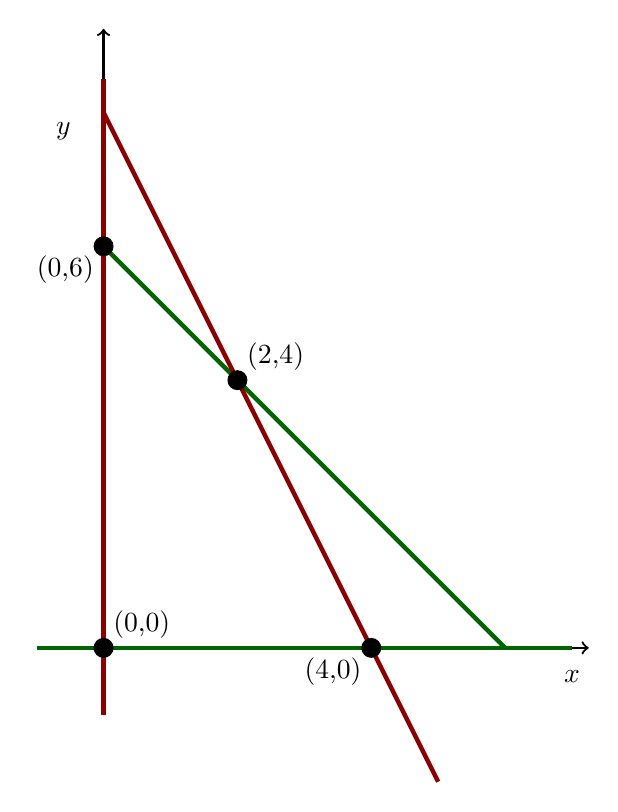
\begin{tikzpicture}[scale=0.85]
        \draw[thick, ->] (-1, 0) -- (7.25, 0);
        \draw[thick, ->] (0, -1) -- (0, 9.25);
        \node[overlay, below] at (7, -0.2) {$x$};
        \node[overlay, below] at (-0.6, 8) {$y$};   
        \draw[ultra thick,DarkGreen, -] (-1, 0) -- (7, 0);        
        \draw[ultra thick,DarkGreen, -] (0,6) -- (6, 0);   
        \draw[ultra thick,DarkRed, -] (0, 8) -- (5, -2);        
        \draw[ultra thick,DarkRed, -] (0, -1) -- (0, 8.5);      
        \filldraw[black] (0,0) circle (4pt) node[anchor=south west]{(0,0)};
        \filldraw[black] (0,6) circle (4pt) node[anchor=north east]{(0,6)};
        \filldraw[black] (2,4) circle (4pt) node[anchor=south west]{(2,4)};
        \filldraw[black] (4,0) circle (4pt) node[anchor=north east]{(4,0)};
        \end{tikzpicture}
        \end{center}            
        } 
        \else 
        \begin{center}
        \begin{tikzpicture}[scale=0.55]
        \draw[very thick, ->] (-6, 0) -- (6.25, 0);
        \draw[very thick, ->] (0, -6) -- (0, 6.25);
        \node[overlay, below] at (6, -0.2) {$x$};
        \node[overlay, below] at (-0.6, 6) {$y$};        
        \end{tikzpicture}
        \end{center}    
    \fi
    \end{parts}
\fi 





\ifnum \Version=2
    \question[6] Consider the non-linear system below.  
    \begin{align*}
        \dxdt &= (x-1)(y-5) , \qquad \dydt = y-x^2-1
    \end{align*}
    \begin{parts}
        \part Determine the locations of the critical points. 
        \ifnum \Solutions=1 {\color{DarkBlue} \\[12pt] 
        For a point to be a critical point, we need $x' = y' = 0$. If $x'$ is zero, then either $x=1$ or $y=5$. 
        \begin{itemize}
            \item When $x=1$, for $y'=0$ we need 
            \begin{align}
                y'&=0 = y - x^2 - 1 \quad \Rightarrow \quad y = 1^2+1 = 2
            \end{align}
            There is a critical point at $(1,2)$. 
            \item When $y=5$, for $y'=0$ we need 
            \begin{align}
                y'&=0 = y - x^2 - 1 \quad \Rightarrow \quad x^2 = 5 - 1 \quad \Rightarrow \quad x = \pm 2
            \end{align}
            There are critical points at $(\pm 2, 5)$.             
        \end{itemize}
            } 
        \else 
        \vfill
        \fi
        \part Sketch the nullclines of the system on the axes below. Clearly indicate the critical points that you found in part (a). 
        \ifnum \Solutions=1 {\color{DarkBlue} \\[12pt] 
        The curves are shown below. The green lines are the x nullclines, and the red curve is the y nullcline. There are exactly three critical points. 
            \begin{center}
            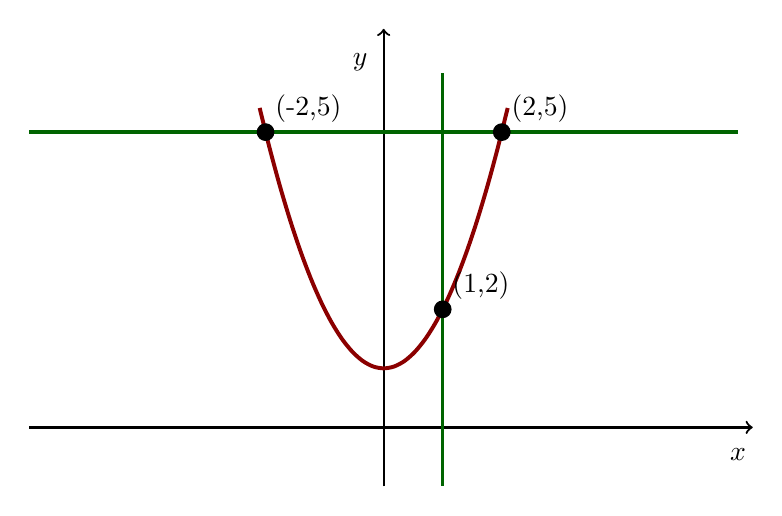
\begin{tikzpicture}[scale=0.75]
            \draw[thick, ->] (-6, 0) -- (6.25, 0);
            \draw[thick, ->] (0, -1) -- (0, 6.75);
            \node[overlay, below] at (6, -0.2) {$x$};
            \node[overlay, below] at (-0.4, 6.5) {$y$};   
            \draw[very thick,DarkGreen, -] (1, 6) -- (1, -1);        
            \draw[very thick,DarkGreen, -] (-6, 5) -- (6, 5);   
            \draw[DarkRed, line width = 0.50mm]   plot[smooth,domain=-2.1:2.1] (\x, {\x*\x+1});
            \filldraw[black] (2,5) circle (4pt) node[anchor=south west]{(2,5)};
            \filldraw[black] (-2,5) circle (4pt) node[anchor=south west]{(-2,5)};
            \filldraw[black] (1,2) circle (4pt) node[anchor=south west]{(1,2)};
            \end{tikzpicture}
            \end{center}               
        } 
        \else 
        \begin{center}
        \begin{tikzpicture}[scale=0.55]
        \draw[very thick, ->] (-6, 0) -- (6.25, 0);
        \draw[very thick, ->] (0, -6) -- (0, 6.25);
        \node[overlay, below] at (6, -0.2) {$x$};
        \node[overlay, below] at (-0.6, 6) {$y$};        
        \end{tikzpicture}
        \end{center}    
    \fi
    \end{parts}
\fi 




\ifnum \Version=3
    \question[6] Consider the non-linear system below.  
    \begin{align*}
        \dxdt &= (x-1)(y-2) , \qquad \dydt = y^2-x
    \end{align*}
    \begin{parts}
        \part Determine the locations of the critical points. 
        \ifnum \Solutions=1 {\color{DarkBlue} \\[12pt] 
        For a point to be a critical point, we need $x' = y' = 0$. If $x'$ is zero, then either $x=1$ or $y=2$. 
        \begin{itemize}
            \item When $x=1$, for $y'=0$ we need 
            \begin{align}
                y'&=0 = y^2 - x \quad \Rightarrow \quad y = \pm 1
            \end{align}
            There are critical points at $(1,\pm 1)$. 
            \item When $y=2$, for $y'=0$ we need 
            \begin{align}
                y'&=0 = y^2 - x  \quad \Rightarrow \quad x = 4 
            \end{align}
            There is a critical point at $(4, 2)$.             
        \end{itemize}
            } 
        \else 
        \vfill
        \fi
        \part Sketch the nullclines of the system on the axes below. Clearly indicate the critical points that you found in part (a). 
        \ifnum \Solutions=1 {\color{DarkBlue} \\[12pt] 
        The curves are shown below. The green lines are the x nullclines, and the red curve is the y nullcline. There are exactly three critical points. 
            \begin{center}
            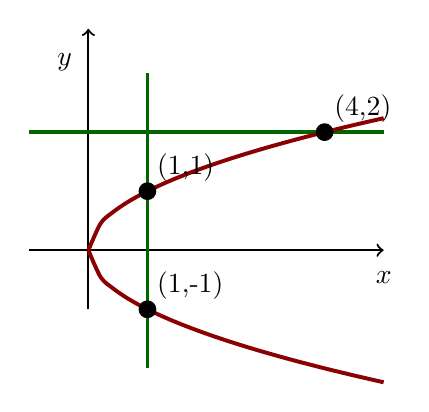
\begin{tikzpicture}[scale=0.75]
            \draw[thick, ->] (-1, 0) -- (5, 0);
            \draw[thick, ->] (0, -1) -- (0, 3.75);
            \node[overlay, below] at (5, -0.2) {$x$};
            \node[overlay, below] at (-0.4, 3.5) {$y$};   
            \draw[very thick,DarkGreen, -] (1, 3) -- (1, -2);        
            \draw[very thick,DarkGreen, -] (-1, 2) -- (5, 2);   
            \draw[DarkRed, line width = 0.50mm]   plot[smooth,domain=0:5] (\x, {\x^(1/2))} );
            \draw[DarkRed, line width = 0.50mm]   plot[smooth,domain=0:5] (\x, {-\x^(1/2))} );
            \filldraw[black] (4,2) circle (4pt) node[anchor=south west]{(4,2)};
            \filldraw[black] (1,1) circle (4pt) node[anchor=south west]{(1,1)};
            \filldraw[black] (1,-1) circle (4pt) node[anchor=south west]{(1,-1)};
            \end{tikzpicture}
            \end{center}               
        } 
        \else 
        \begin{center}
        \begin{tikzpicture}[scale=0.55]
        \draw[very thick, ->] (-6, 0) -- (6.25, 0);
        \draw[very thick, ->] (0, -6) -- (0, 6.25);
        \node[overlay, below] at (6, -0.2) {$x$};
        \node[overlay, below] at (-0.6, 6) {$y$};        
        \end{tikzpicture}
        \end{center}    
    \fi
    \end{parts}
\fi 


\ifnum \Version=6
    \question[4] Consider the non-linear system below.  
    \begin{align*}
        \dxdt &= (x-2)(y-1) , \qquad \dydt = 2y^2-x
    \end{align*}
    \begin{parts}
        \part Determine the locations of the critical points. 
        \ifnum \Solutions=1 {\color{DarkBlue} \\[12pt] 
        For a point to be a critical point, we need $x' = y' = 0$. If $x'$ is zero, then either $x=2$ or $y=1$. 
        \begin{itemize}
            \item When $x=2$, for $y'=0$ we need 
            \begin{align}
                y'&=0 = 2y^2 - x \quad \Rightarrow \quad y = \pm 1
            \end{align}
            There are critical points at $(2,\pm 1)$. 
            \item When $y=1$, for $y'=0$ we need 
            \begin{align}
                y'&=0 = 2y^2 - x  \quad \Rightarrow \quad x = 2
            \end{align}
            There is a critical point at $(2,1)$, which we already had.          
        \end{itemize}
            } 
        \else 
        \vfill
        \fi
        \part Sketch the nullclines of the system on the axes below. Clearly indicate the critical points that you found in part (a). 
        \ifnum \Solutions=1 {\color{DarkBlue} \\[12pt] 
        The curves are shown below. The green lines are the x nullclines, and the red curve is the y nullcline. There are exactly three critical points. 
            \begin{center}
            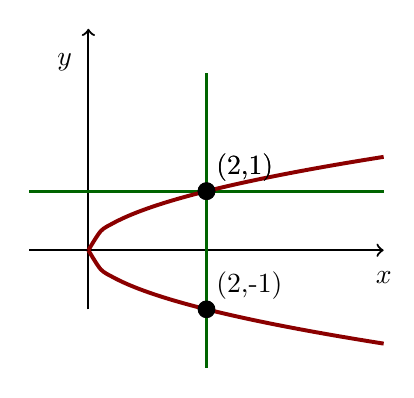
\begin{tikzpicture}[scale=0.75]
            \draw[thick, ->] (-1, 0) -- (5, 0);
            \draw[thick, ->] (0, -1) -- (0, 3.75);
            \node[overlay, below] at (5, -0.2) {$x$};
            \node[overlay, below] at (-0.4, 3.5) {$y$};   
            \draw[very thick,DarkGreen, -] (2, 3) -- (2, -2);        
            \draw[very thick,DarkGreen, -] (-1, 1) -- (5, 1);   
            \draw[DarkRed, line width = 0.50mm]   plot[smooth,domain=0:5] (\x, {(\x/2)^(1/2))} );
            \draw[DarkRed, line width = 0.50mm]   plot[smooth,domain=0:5] (\x, {-(\x/2)^(1/2))} );
            \filldraw[black] (2,1) circle (4pt) node[anchor=south west]{(2,1)};
            \filldraw[black] (2,1) circle (4pt) node[anchor=south west]{(2,1)};
            \filldraw[black] (2,-1) circle (4pt) node[anchor=south west]{(2,-1)};
            \end{tikzpicture}
            \end{center}               
        } 
        \else 
        \begin{center}
        \begin{tikzpicture}[scale=0.55]
        \draw[very thick, ->] (-6, 0) -- (6.25, 0);
        \draw[very thick, ->] (0, -6) -- (0, 6.25);
        \node[overlay, below] at (6, -0.2) {$x$};
        \node[overlay, below] at (-0.6, 6) {$y$};        
        \end{tikzpicture}
        \end{center}    
    \fi
    \end{parts}
\fi 


\ifnum \Version=7
    \question[4] Consider the non-linear system below.  
    \begin{align*}
        \dxdt &= (x-1)(y-5) , \qquad \dydt = y-x^2-1
    \end{align*}
    \begin{parts}
        \part Determine the locations of the critical points. 
        \ifnum \Solutions=1 {\color{DarkBlue} \\[12pt] 
        For a point to be a critical point, we need $x' = y' = 0$. If $x'$ is zero, then either $x=1$ or $y=5$. 
        \begin{itemize}
            \item When $x=1$, for $y'=0$ we need 
            \begin{align}
                y'&=0 = y - x^2 - 1 \quad \Rightarrow \quad y = 1^2+1 = 2
            \end{align}
            There is a critical point at $(1,2)$. 
            \item When $y=5$, for $y'=0$ we need 
            \begin{align}
                y'&=0 = y - x^2 - 1 \quad \Rightarrow \quad x^2 = 5 - 1 \quad \Rightarrow \quad x = \pm 2
            \end{align}
            There are critical points at $(\pm 2, 5)$.             
        \end{itemize}
            } 
        \else 
        \vfill
        \fi
        \part Sketch the nullclines of the system on the axes below. Clearly indicate the critical points that you found in part (a). 
        \ifnum \Solutions=1 {\color{DarkBlue} \\[12pt] 
        The curves are shown below. The green lines are the x nullclines, and the red curve is the y nullcline. There are exactly three critical points. 
            \begin{center}
            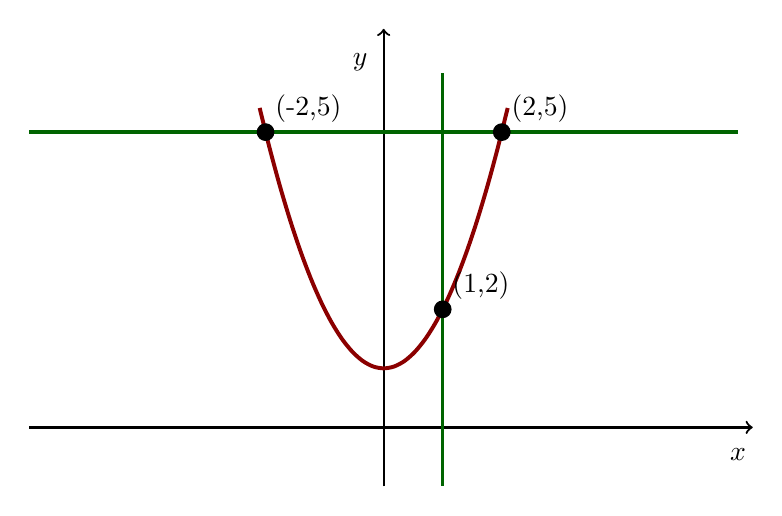
\begin{tikzpicture}[scale=0.75]
            \draw[thick, ->] (-6, 0) -- (6.25, 0);
            \draw[thick, ->] (0, -1) -- (0, 6.75);
            \node[overlay, below] at (6, -0.2) {$x$};
            \node[overlay, below] at (-0.4, 6.5) {$y$};   
            \draw[very thick,DarkGreen, -] (1, 6) -- (1, -1);        
            \draw[very thick,DarkGreen, -] (-6, 5) -- (6, 5);   
            \draw[DarkRed, line width = 0.50mm]   plot[smooth,domain=-2.1:2.1] (\x, {\x*\x+1});
            \filldraw[black] (2,5) circle (4pt) node[anchor=south west]{(2,5)};
            \filldraw[black] (-2,5) circle (4pt) node[anchor=south west]{(-2,5)};
            \filldraw[black] (1,2) circle (4pt) node[anchor=south west]{(1,2)};
            \end{tikzpicture}
            \end{center}               
        } 
        \else 
        \begin{center}
        \begin{tikzpicture}[scale=0.55]
        \draw[very thick, ->] (-6, 0) -- (6.25, 0);
        \draw[very thick, ->] (0, -6) -- (0, 6.25);
        \node[overlay, below] at (6, -0.2) {$x$};
        \node[overlay, below] at (-0.6, 6) {$y$};        
        \end{tikzpicture}
        \end{center}    
    \fi
    \end{parts}
\fi 

        \ifnum \Solutions=0
\newpage 
\fi
\ifnum \Version=1
\question[5] Consider the non-linear system below.  
\begin{align*}
    \dxdt &= x^2+y-2x-12 , \qquad \dydt = y-x-6
\end{align*}
The critical points are located at $(-2,4)$ and $(3,9)$. 
\begin{parts}
    \part Compute the Jacobian matrix, $J$, for the approximating linear system. 
    \ifnum \Solutions=1 {\color{DarkBlue}
        \begin{align}
            F &= x'\\
            G &= y' \\
            J &= \begin{pmatrix} F_x&F_y\\ G_x & G_y\end{pmatrix} = \begin{pmatrix} 2x-2&1\\-1&1\end{pmatrix}
        \end{align}
        } 
    \else 
    \vfill
    \fi        
    \part Use eigenvalues to classify the critical point at $(-2,4)$ according to stability (stable, unstable, asymptotically stable) and type (saddle, proper node, etc).
    \ifnum \Solutions=1 {\color{DarkBlue} \\[12pt] 
        At $(-2,4)$, $J = \begin{pmatrix} -6&1\\-1&1\end{pmatrix}$. The eigenvalues are the roots of \begin{align}
            (-6-\lambda)(1-\lambda)+1 = \lambda^2 +5\lambda - 5
        \end{align}
        Thus 
        \begin{align}
            \lambda = -\frac52 \pm \frac12 \sqrt{25-4\cdot(-5)} = -\frac52 \pm \frac{\sqrt{45}}{2}
        \end{align}
        $\lambda \in \mathbb R$, and the eigenvalues have opposite signs. The critical point is an unstable saddle. 
        } 
    \else 
    \vfill
    \fi
    \part Use eigenvalues to classify the critical point at $(3,9)$ according to stability (stable, unstable, asymptotically stable) and type (saddle, proper node, etc).
    \ifnum \Solutions=1 {\color{DarkBlue} \\[12pt] 
        At $(3,9)$, $J = \begin{pmatrix} 4&1\\-1&1\end{pmatrix}$. The eigenvalues are the roots of \begin{align}
            (4-\lambda)(1-\lambda)+1 = \lambda^2 - 5\lambda +5 
        \end{align}
        Thus 
        \begin{align}
            \lambda = \frac52 \pm \frac12 \sqrt{25-4\cdot(5)} = \frac52 \pm \frac{\sqrt{5}}{2}
        \end{align}
        $\lambda \in \mathbb R$, and the eigenvalues both positive. The critical point is an unstable node. 
    } 
    \else 
    \vfill
\fi
\end{parts}
\fi



\ifnum \Version=2
\question[6] Consider the non-linear system below.  
\begin{align*}
    \dxdt &= x(1-x-y) , \qquad \dydt = y(2-x-y)
\end{align*}
The critical points are located at $(0,0)$, $(0,2)$, and $(1,0)$. 
\begin{parts}
    \part Compute the Jacobian matrix, $J$, for the approximating linear system. 
    \ifnum \Solutions=1 {\color{DarkBlue} \\
    Set $ F = x'$ and $G = y'$. Then
        \begin{align}
            F_x &= 1 - 2x -y\\
            F_y &= -x \\
            G_x &= 2-x-2y \\
            G_y &= -y \\
            J &= \begin{pmatrix} F_x&F_y\\ G_x & G_y\end{pmatrix} = \begin{pmatrix} -1-x-2y & -x\\-y&2-x-2y \end{pmatrix}
        \end{align}
        } 
    \else 
    \vfill
    \fi        
    \part Use eigenvalues to classify the critical point at $(0,0)$ according to stability (stable, unstable, asymptotically stable) and type (saddle, proper node, etc).
    \ifnum \Solutions=1 {\color{DarkBlue} \\[12pt] 
        At $(0,0)$, $J = \begin{pmatrix} 1&0\\0&2\end{pmatrix}$. The eigenvalues are $\lambda = 1,2$. \\ Thus the critical point is an \textbf{unstable node}. 
        } 
    \else 
    \vfill
    \fi
    \part Use eigenvalues to classify the critical point at $(0,2)$ according to stability (stable, unstable, asymptotically stable) and type (saddle, proper node, etc).
    \ifnum \Solutions=1 {\color{DarkBlue} \\[12pt] 
        At $(0,2)$, $J = \begin{pmatrix} -1&0\\-2&-4\end{pmatrix}$. The eigenvalues are $\lambda = -1,-4$. \\Thus the critical point is a \textbf{stable node}. 
        } 
    \else 
    \vfill
    \fi
    \part Use eigenvalues to classify the critical point at $(1,0)$ according to stability (stable, unstable, asymptotically stable) and type (saddle, proper node, etc).
    \ifnum \Solutions=1 {\color{DarkBlue} \\[12pt] 
        At $(1,0)$, $J = \begin{pmatrix} -1&-1\\0&1\end{pmatrix}$. The eigenvalues are $\lambda = \pm 1$. \\ Thus the critical point is an \textbf{unstable saddle}. 
        } 
    \else 
    \vfill
    \fi    
\end{parts}
\fi










\ifnum \Version>5
\question[6] Consider the non-linear system below.  
\begin{align*}
    \dxdt &= x(4-x-y) , \qquad \dydt = y(6-2x-y)
\end{align*}
\begin{parts}
    \part Compute the Jacobian matrix, $J$, for the approximating linear system. 
    \ifnum \Solutions=1 {\color{DarkBlue} \\
    Set $ F = x'$ and $G = y'$. Then
        \begin{align}
            F &= 4x - x^2 - xy \\
            G &= 6y -2xy - y^2 \\
            J &= \begin{pmatrix} F_x&F_y\\ G_x & G_y\end{pmatrix} 
            = \begin{pmatrix} 4-2x-y & -x\\-2y& 6-2x-2y \end{pmatrix}
        \end{align}
        } 
    \else 
    \vfill
    \fi        
    \part Use eigenvalues to classify the critical point at $(0,6)$ according to stability (stable, unstable, asymptotically stable) and type (saddle, proper node, etc).
    \ifnum \Solutions=1 {\color{DarkBlue} \\[12pt] 
        At $(0,0)$, $J = \begin{pmatrix} -2&0\\-12&-6\end{pmatrix}$. The eigenvalues are $\lambda = -2, -6$. The CP is a \textbf{stable node}. 
        } 
    \else 
    \vfill
    \fi
    \part Use eigenvalues to classify the critical point at $(2,2)$ according to stability (stable, unstable, asymptotically stable) and type (saddle, proper node, etc).
    \ifnum \Solutions=1 {\color{DarkBlue} \\[12pt] 
        At $(0,2)$, $J = \begin{pmatrix} -2&-2\\-4&-2\end{pmatrix}$. Eigenvalues:
        \begin{align}
            0 &= (\lambda + 2)^2 - 8 = \lambda^2 + 4\lambda -4  \\
            \lambda &= -2 \pm \frac12 \sqrt{16 + 16} = -2 \pm 2\sqrt 2
        \end{align}\\Thus the critical point is an \textbf{unstable saddle}. 
        } 
    \else 
    \vfill
    \fi
\end{parts}
\fi


        \ifnum \Solutions=0
\newpage 
\fi
\ifnum \Version=1    
    \question[6] Use the Laplace transform to solve the following IVP. Do not leave your answer in terms of an integral. Please show your work.
    % $$\displaystyle y''-4y'+4y=0,\qquad y(0)=1,\quad y'(0)=1$$ %Q,A HW 5.4#4
    % $$\displaystyle y''-2y'+4y=0,\qquad y(0)=2,\quad y'(0)=0$$ %M HW 5.4#5
    $$ y'' -6y'+13y = 0, \quad y(0) = 0, \quad y'(0) = -3$$. % A TRIM P301 #27
    % $$ y''+ 2y'+y = 0, \quad y(0) = 1, \quad y'(0) = 1$$. % B TRIM P301 #23
\ifnum \Solutions=1 {\color{DarkBlue} 
Take the transform of the DE and solve for $Y(s) = \mathcal{L}[y(t)]$.
\begin{align}
    0
    &= s^2Y-sy(0) - y'(0) - 6(sY-y(0)) + 13Y \\
    &= s^2Y-0 +3 - 6(sY-0) + 13Y \\
    -3 &= s^2Y - 6sY + 13Y \\
    -3 &= (s^2 - 6s + 13)Y \\
    Y &= \frac{-3}{s^2- 6s+13} 
\end{align}    
Complete the square:
\begin{align}
    Y &= \frac{-3}{s^2- 6s+9-9+13} = \frac{-3}{ (s-3)^2+4}=\frac{-3}{2}\cdot \frac{2}{ (s-3)^2+4}
\end{align}    
Inverse transform:
\begin{align}
    y(t) &= \frac{-3}{2}\sin(2t)e^{3t}
\end{align}
} 
\else 
\vspace{3cm}
\fi
\fi 



\ifnum \Version=2
    \question[6] Consider the IVP: $y''+4y'+3y = 4e^{-2t}$, $y(0)=0, y'(0) = 0$. 
        \begin{parts}
        \part Use the Laplace Transform to obtain an explicit expression for $Y(s) = \mathcal{L}[y]$. 
        \ifnum \Solutions=1 {\color{DarkBlue} \\[12pt] 
        Taking the transform of the IVP yields
        \begin{align}
            s^2Y-sy(0) - y'(0) +4(sY-y(0)) +3 Y &= \frac{4}{s+2} \\
            (s^2 +4s+3)Y &= \frac{4}{s+2} \\
            Y&= \frac{1}{s+2} \frac{4}{s^2 +4s+3} \\
            &= \frac{4}{(s+1)(s+2)(s+3)}
        \end{align}
        } 
        \else 
        \vfill
        \fi
        \part Use the inverse Laplace Transform to solve the IVP. 
        \ifnum \Solutions=1 {\color{DarkBlue} \\[12pt] 
        Partial fractions: 
        \begin{align}
            \frac{4}{(s+2)(s+1)(s+3)} & = \frac{A}{s+1} + \frac{B}{s+2} + \frac{C}{s+3} \\
            4 & = A(s+2)(s+3) + B(s+1)(s+3) + C(s+1)(s+2) 
        \end{align}
        Selecting values of $s$ yields
        \begin{align}
            s=-1: \quad 4 & = 2A + 0 + 0 \quad \Rightarrow \quad A = 2 \\
            s=-2: \quad 4 & = 0 - B + 0 \quad \Rightarrow \quad B = -4 \\
            s=-3: \quad 4 & = 0 + 0 + 2C \quad \Rightarrow \quad C = 2
        \end{align}
        Thus
       \begin{align}
            Y (s) = \frac{4}{(s+1)(s+2)(s+3)} 
            &= \frac{A}{s+1} + \frac{B}{s+2} + \frac{C}{s+3} \\
            &= \frac{2}{s+1} + \frac{-4}{s+2} + \frac{2}{s+3} 
        \end{align}        
        With the inverse transform this becomes 
        \begin{align}
            y(t) &= 2e^{-t} -4 e^{-2t} +2 e^{-3t}
        \end{align}
        } 
        \else 
        \vfill
        \fi
    \end{parts}
\fi 




\ifnum \Version>5
    \question[4] Consider the IVP: $y''+4y = 8e^{-2t}$, $y(0)=0, y'(0) = 0$. 
        \begin{parts}
        \part Use the Laplace Transform to obtain an explicit expression for $Y(s) = \mathcal{L}[y]$. 
        \ifnum \Solutions=1 {\color{DarkBlue} \\[12pt] 
        Taking the transform of the IVP yields
        \begin{align}
            s^2Y-sy(0) - y'(0) + 4 Y &= \frac{8}{s+2} \\
            (s^2 + 4)Y &= \frac{8}{s+2} \\
            Y&= \frac{8}{s+2} \frac{1}{s^2 + 4} \\
            &= \frac{8}{(s^2+4)(s+2)}
        \end{align}
        } 
        \else 
        \vfill
        \fi
        \part Use the inverse Laplace Transform to solve the IVP. 
        \ifnum \Solutions=1 {\color{DarkBlue} \\[12pt] 
        Partial fractions: 
        \begin{align}
            \frac{8}{(s^2+4)(s+2)} & = \frac{As+B}{s^2+4} + \frac{C}{s+2} \\
            8 & = (As+B)(s+2) + C(s^2+4) \\
            8 &= (A+C)s^2 +(2A+B)s+(2B+4C)
        \end{align}
        Selecting $s = -2$ yields
        \begin{align}
            s=-2: \quad 8 & = 0 + C((-2)^2+4) \quad \Rightarrow \quad C = 1 
        \end{align}
        The quadratic terms give us 
        \begin{align}
            A+C = 0 \Rightarrow \quad A = - 1 
        \end{align}
        The linear terms give us 
        \begin{align}
            2A+B = 0 \Rightarrow \quad B = 2
        \end{align}        
        Thus
       \begin{align}
            Y (s) = \frac{8}{(s^2+4)(s+2)} 
            &= \frac{As+B}{s^2+4} + \frac{C}{s+2} \\
            &= \frac{-s+2}{s^2+4} + \frac{1}{s+2} \\
            &= -\frac{s}{s^2+4} + \frac{2}{s^2+4} + \frac{1}{s+2} \\
        \end{align}        
        With the inverse transform this becomes 
        \begin{align}
            y(t) &= \sin(2t) - \cos(2t) + e^{-2t}
        \end{align}
        \textbf{Additional Notes}\\
        Some students made an error in taking the transform that resulted in the expression
        $$Y = \frac{8}{s(s+4)(s+2)} = \frac1s+\frac{1}{s+4}- \frac{2}{s+2}$$
        } 
        \else 
        \vfill
        \fi
    \end{parts}
\fi 


        \ifnum \Solutions=0
\newpage 
\fi

\ifnum \Version=1    
\question[2] 
Compute the Laplace transform of the function below. Do not leave your answer in terms of an integral. Please show your work. 
$$y(t) = \begin{cases} 0, \quad 0 \le t < 1 \\ t-2, \quad 1 \le t < 3 \\ 0, \quad 3 \le t < \infty\end{cases}$$
\ifnum \Solutions=1 {\color{DarkBlue} \\[12pt] 
There are a few different ways to solve this. Any of the approaches below are sufficient. 
\subsection*{Method 1: Direct Integration }
Direct integration requires integration by parts, but using the definition of the Laplace Transform:
    \begin{align}
        \int_0^{\infty} e^{-st} y(t) \, dt 
        &= \int_1^{3} e^{-st} \, (t-2) \, dt \\
        &= \int_1^{3} te^{-st}  \, dt - 2 \int_1^{3} e^{-st}  \, dt \\
        &=  \left. t\cdot \frac{-1}{s}e^{-st} \right|_1^3
        - \int_1^{3} \frac{-1}{s}e^{-st} \, dt 
        -2 \left( \left. \frac{-1}{s}e^{-st}\right|_{t=1}^{t=3}\right) \\
        &=  \frac{-1}{s}\left( 3e^{-3s} - e^{-s} \right)  
        + \frac{1}{s} \int_1^{3} e^{-st} \, dt 
        + \frac{2}{s} \left(  e^{-3s} - e^{-s} \right) \\
        &=  \frac{-1}{s}\left( 3e^{-3s} - e^{-s} \right)  
        + \frac{1}{s} \left( \left. \frac{-1}{s}e^{-st}\right|_{t=1}^{t=3}\right) \, dt 
        + \frac{2}{s} \left(  e^{-3s} - e^{-s} \right) \\     
        &=  \frac{-1}{s}\left( 3e^{-3s} - e^{-s} \right)  
        - \frac{1}{s^2} \left(  e^{-3s} - e^{-s} \right) 
        + \frac{2}{s} \left(  e^{-3s} - e^{-s} \right) \\      
        &= - \frac{1}{s^2} \left(  e^{-3s} - e^{-s} \right) 
        - \frac{ e^{-3s}}{s}   - \frac{e^{-s}}{s}  \\   
        &= \frac{e^{-s}}{s^2} - \frac{e^{-3s}}{s^2} 
        - \frac{ e^{-3s}}{s}   - \frac{e^{-s}}{s}           
    \end{align}
    \subsection*{Method 2: Step Functions}
    We could also use the table of transforms, specifically the transform of the step function $u_c(t)$ and its product with another function. 
    \begin{align}
        y(t) &= 0u_{0,1} + (t-2)u_{1,3} + 0u_{3} 
        =(t-2)(u_1-u_3) 
        = tu_1-tu_3 - 2u_1 + 2 u_3 
    \end{align}   
    At this point we can either take the transform and use the derivative theorem (in the table) to work out the transform of $tu_1$ and $tu_3$, or we can use the following trick:
    \begin{align}
        y(t) &= tu_1-tu_3 - 2u_1 + 2 u_3 \\
        &= (t+1-1)u_1-(t+3-3)u_3 - 2u_1 + 2 u_3 \\
        &= (t-1)u_1 + u_1 -(t-3)u_3 - 3u_3 - 2u_1 + 2 u_3 \\
        &= (t-1)u_1 -(t-3)u_3 - u_1 - u_3 
    \end{align}
    Using the table of transforms the Laplace transform is
    \begin{align}
        Y(s) = \frac{e^{-s}}{s^2} - \frac{e^{-3s}}{s^2} - \frac{e^{-s}}{s} - \frac{e^{-3s}}{s}
    \end{align}
} 
\else 
    \vfill
    \begin{center}
        \textit{This remainder of this page can be used for scratch work. }
    \end{center}
    \vfill
\fi
\fi


\ifnum \Version=5
\question[2] 
Compute the Laplace transform of the function below. Do not leave your answer in terms of an integral. Please show your work. 
$$y(t) = \begin{cases} 0, \quad 0 \le t < 1 \\ 4, \quad 1 \le t < 3 \\ 0, \quad 3 \le t < \infty\end{cases}$$
\ifnum \Solutions=1 {\color{DarkBlue} \\[12pt] 
There are a few different ways to solve this. Any of the approaches below are sufficient. 
\subsection*{Method 1: Direct Integration }
Direct integration uses the definition of the Laplace Transform:
    \begin{align}
        \int_0^{\infty} e^{-st} y(t) \, dt 
        = \int_1^{3} e^{-st} \, 4 \, dt 
        &= 4\int_1^{3} e^{-st}  \, dt  \\         
        &= 4\left.\frac{-1}{s} e^{-st} \right|_1^3  \\         
        &= \frac{-4}{s} \left(e^{-3s}  - e^{-s} \right)     
    \end{align}
    \subsection*{Method 2: Step Functions}
    We could also use the table of transforms, specifically the transform of the step function $u_c(t)$ and its product with another function. 
    \begin{align}
        y(t) &= 0u_{0,1} + 4u_{1,3} + 0u_{3} 
        =4(u_1-u_3) 
        = 4u_1 - 4 u_3 
    \end{align}   
    Using the table of transforms the Laplace transform is
    \begin{align}
        Y(s) = 4 \frac{e^{-s}}{s} - 4\frac{e^{-3s}}{s}
    \end{align}
    \newpage
} 
\else 
    \vfill
    \begin{center}
        \textit{This remainder of this page can be used for scratch work. }
    \end{center}
    \vfill
\fi
\fi







\ifnum \Version=6
\question[3] 
The function $f(t)$ is periodic, has period $4$, and 
        $$f(t) = \begin{cases} e^{-3t}, \quad 0 \le t < 2 \\ 0, \quad 2 \le t < 4 \end{cases}$$
        Compute the Laplace transform of $f(t)$. Do not leave your answer in terms of an integral. Please show your work. 

\ifnum \Solutions=1 {\color{DarkBlue} 
    We use the formula for a periodic function with $T=4$. 
    
        With $T=4$,
        
        \begin{align}
            \mathcal{L}\{f(t)\} &=  \frac{\int_{0}^{T} e^{-st} f(t) dt}{1 - e^{-Ts}} \\
            &= \frac{1}{1 - e^{-4s}} \left( \int_{0}^{2} e^{-st} e^{-3t} dt + \int_2^4 0 \, dt \right)\\
            &= \frac{1}{1 - e^{-4s}} \cdot \frac{1}{-s-3} \left. e^{(-s-3)t}\right|_0^2 \\
            &= -\frac{1}{1 - e^{-4s}} \cdot \frac{1}{s+3} \left( e^{-2(s+3)} - 1 \right)
        \end{align}
        \newpage
} 
\else 
    \newpage
    \begin{center}
        \textit{This remainder of this page can be used for scratch work. }
    \end{center}
    \vfill
\fi
\fi



\ifnum \Version=7
\question[3] 
The function $f(t)$ is periodic, has period $4$, and 
        $$f(t) = \begin{cases} e^{-2t}, \quad 0 \le t < 3 \\ 0, \quad 3 \le t < 4 \end{cases}$$
        Compute the Laplace transform of $f(t)$. Do not leave your answer in terms of an integral. Please show your work. 

\ifnum \Solutions=1 {\color{DarkBlue} 
    We use the formula for a periodic function with $T=4$. 
    
        With $T=4$,
        
        \begin{align}
            \mathcal{L}\{f(t)\} &=  \frac{\int_{0}^{T} e^{-st} f(t) dt}{1 - e^{-Ts}} \\
            &= \frac{1}{1 - e^{-4s}} \left( \int_{0}^{3} e^{-st} e^{-2t} dt + \int_3^4 0 \, dt \right)\\
            &= \frac{1}{1 - e^{-4s}} \cdot \frac{1}{-s-2} \left. e^{(-s-2)t}\right|_0^3 \\
            &= -\frac{1}{1 - e^{-4s}} \cdot \frac{1}{s+2} \left( e^{-3(s+2)} - 1 \right)
        \end{align}
} 
\else 
    \newpage
    \begin{center}
        \textit{This remainder of this page can be used for scratch work. }
    \end{center}
    \vfill
\fi
\fi




    \fi 
    
    \ifnum \Set=2
        \newpage 

\ifnum \Version=1    
\question[10] Consider the first order linear system of differential equations $\vec x \, ' = A\vec x$, where $\vec x = \vec x(t)$, and 

$$A = \begin{pmatrix} 0&2&1 \\ 1&-1&-1 \\ 1&-2&0 \end{pmatrix}$$

The eigenvalues of $A$ are $\lambda_1 = \lambda_2 = 1$, and $\lambda_3 = -3$. 

\begin{parts}
    \part Determine the eigenvectors of $A$. Please show your work. 
    \vspace{10cm}
    \part Write down the general solution to the system of differential equations using your results from Part (a).
\end{parts}
\fi

\ifnum \Version=2
\question[10] Consider the first order, constant coefficient, linear initial value problem $\vec x \, ' = A\vec x, \ \vec x (0) = \vec x_0$, where $\vec x \, ' = A\vec x$ and $\vec x = \vec x(t)$. The vector $\vec x_0$, and the eigenvalues and eigenvectors of $A$ are as follows. 
$$\lambda_1 = -4, \ \vec v_1 = \begin{pmatrix}1\\0\\0\end{pmatrix} , \quad \lambda_2 = -4, \ \vec v_2 = \begin{pmatrix} 0\\1\\2 \end{pmatrix}, \quad \lambda_3 = -12, \ \vec v_3 = \begin{pmatrix} 0\\0\\1\end{pmatrix}, \quad \vec x_0 = \begin{pmatrix} 8\\4\\10\end{pmatrix}$$
\begin{parts}
    \part Write down the general solution to the system of differential equations $\vec x \, ' = A \vec x$ in terms of real-valued functions. 
    \vspace{4cm}
    \part Solve the initial value problem. Please state the solution to the initial value problem clearly and please show your work. 
\end{parts}
\fi


\ifnum \Version=3
\question[10] Consider the first order, constant coefficient, linear initial value problem $\vec x \, ' = A\vec x, \ \vec x (0) = \vec x_0$, where $\vec x \, ' = A\vec x$ and $\vec x = \vec x(t)$. The vector $\vec x_0$, and the eigenvalues and eigenvectors of $A$ are as follows. 
$$\lambda_1 = -4, \ \vec v_1 = \begin{pmatrix}1\\0\\0 \end{pmatrix} , \quad \lambda_2 = -2, \ \vec v_2 = \begin{pmatrix} 3\\1\\0 \end{pmatrix}, \quad \lambda_3 = -2, \ \vec v_3 = \begin{pmatrix} -1\\0\\2\end{pmatrix}, \quad \vec x_0 = \begin{pmatrix} 9\\4\\10\end{pmatrix}$$
\begin{parts}
    \part Write down the general solution to the system of differential equations $\vec x \, ' = A \vec x$ in terms of real-valued functions. 
    \vspace{4cm}
    \part Solve the initial value problem. Please state the solution to the initial value problem clearly and please show your work. 
\end{parts}
\fi


\ifnum \Version=6
\question[10] Consider the first order, constant coefficient, linear initial value problem $\vec x \, ' = A\vec x, \ \vec x (0) = \vec x_0$, where $\vec x \, ' = A\vec x$ and $\vec x = \vec x(t)$. The vector $\vec x_0$, and the eigenvalues and eigenvectors of $A$ are as follows. 
$$\lambda_1 = -4, \ \vec v_1 = \begin{pmatrix}1\\2\\0 \end{pmatrix} , \quad \lambda_2 = -4, \ \vec v_2 = \begin{pmatrix} 0\\1\\3 \end{pmatrix}, \quad \lambda_3 = -2, \ \vec v_3 = \begin{pmatrix} 0\\0\\1\end{pmatrix}, \quad \vec x_0 = \begin{pmatrix} 3\\4\\12\end{pmatrix}$$
\begin{parts}
    \part Write down the general solution to the system of differential equations $\vec x \, ' = A \vec x$ in terms of real-valued functions. 
    
    \ifnum \Solutions=1 {\color{DarkBlue}
    \textbf{Solutions:}
    \begin{align}
        \vec x &= 
        c_1 e^{-4t} \begin{pmatrix} 1\\2\\0  \end{pmatrix} + 
        c_2 e^{-4t} \begin{pmatrix} 0\\1\\3  \end{pmatrix} + 
        c_3 e^{-2t} \begin{pmatrix} 0\\0\\1 \end{pmatrix}
    \end{align}
    } 
    \else 
        \vspace{4cm}
\fi
    \part Solve the initial value problem. Please state the solution to the initial value problem clearly and please show your work. 
    
\ifnum \Solutions=1 {\color{DarkBlue} 
\textbf{Solutions:} at $t=0$, 
    \begin{align}
        \vec x &= 
        \begin{pmatrix} 3\\4\\12 \end{pmatrix} = 
        c_1  \begin{pmatrix} 1\\2\\0  \end{pmatrix} + 
        c_2  \begin{pmatrix} 0\\1\\3  \end{pmatrix} + 
        c_3  \begin{pmatrix} 0\\0\\1 \end{pmatrix}
    \end{align}
    Forming an augmented matrix and row reducing: 
    \begin{align}
        \begin{pmatrix} 1&0&0&3 \\ 2&1&0 & 4 \\ 0&3&1&12 \end{pmatrix} 
        \sim \begin{pmatrix} 1&0&0&3 \\ 0&1&0 & -2 \\ 0&3&1&12 \end{pmatrix} 
        \sim \begin{pmatrix} 1&0&0&3 \\ 0&1&0 & -2 \\ 0& 0 &1&18 \end{pmatrix} 
    \end{align}
    The solution is
    \begin{align}
        \vec x &= 
        3 e^{-4t} \begin{pmatrix} 1\\2\\0  \end{pmatrix} 
        -2 e^{-4t} \begin{pmatrix} 0\\1\\3  \end{pmatrix} 
        +18 e^{-2t} \begin{pmatrix} 0\\0\\1 \end{pmatrix}
    \end{align}    
} 
\else 
\fi    
\end{parts}
\fi


\ifnum \Version=7
\question[10] Consider the first order, constant coefficient, linear initial value problem $\vec x \, ' = A\vec x, \ \vec x (0) = \vec x_0$, where $\vec x \, ' = A\vec x$ and $\vec x = \vec x(t)$. The vector $\vec x_0$, and the eigenvalues and eigenvectors of $A$ are as follows. 
$$\lambda_1 = -2, \ \vec v_1 = \begin{pmatrix}1\\3\\0 \end{pmatrix} , \quad \lambda_2 = -2, \ \vec v_2 = \begin{pmatrix} 0\\1\\2 \end{pmatrix}, \quad \lambda_3 = -3, \ \vec v_3 = \begin{pmatrix} 0\\0\\1\end{pmatrix}, \quad \vec x_0 = \begin{pmatrix} 3\\4\\2\end{pmatrix}$$
\begin{parts}
    \part Write down the general solution to the system of differential equations $\vec x \, ' = A \vec x$ in terms of real-valued functions. 
    \ifnum \Solutions=1 {\color{DarkBlue}
    \textbf{Solutions:}
    \begin{align}
        \vec x &= 
        c_1 e^{-2t} \begin{pmatrix} 1\\3\\0  \end{pmatrix} + 
        c_2 e^{-2t} \begin{pmatrix} 0\\1\\2  \end{pmatrix} + 
        c_3 e^{-3t} \begin{pmatrix} 0\\0\\1 \end{pmatrix}
    \end{align}
    } 
    \else 
        \vspace{4cm}
\fi
    \part Solve the initial value problem. Please state the solution to the initial value problem clearly and please show your work. 
    
\ifnum \Solutions=1 {\color{DarkBlue} 
\textbf{Solutions:} at $t=0$, 
    \begin{align}
        \vec x &= 
        \begin{pmatrix} 3\\4\\2 \end{pmatrix} = 
        c_1  \begin{pmatrix} 1\\3\\0  \end{pmatrix} + 
        c_2  \begin{pmatrix} 0\\1\\2  \end{pmatrix} + 
        c_3  \begin{pmatrix} 0\\0\\1 \end{pmatrix}
    \end{align}
    Forming an augmented matrix and row reducing: 
    \begin{align}
        \begin{pmatrix} 1&0&0&3 \\ 3&1&0 & 4 \\ 0&2&1&2 \end{pmatrix} 
        \sim \begin{pmatrix} 1&0&0&3 \\ 0&1&0 & -5 \\ 0&2&1&2 \end{pmatrix} 
        \sim \begin{pmatrix} 1&0&0&3 \\ 0&1&0 & -5 \\ 0& 0 &1&12 \end{pmatrix} 
    \end{align}
    The solution is
    \begin{align}
        \vec x &= 
        3 e^{-4t} \begin{pmatrix} 1\\3\\0  \end{pmatrix} 
        -5 e^{-4t} \begin{pmatrix} 0\\1\\2  \end{pmatrix} 
        +12 e^{-2t} \begin{pmatrix} 0\\0\\1 \end{pmatrix}
    \end{align}    
} 
\else 
\fi    
\end{parts}
\fi

        
        \ifnum \Version=1
\question[2] State a suitable form for the particular solution if the method of undetermined coefficients is to be used to solve  $y'' + 7y' + 12y=t^2e^{-3t}$. Please show your work for this question. 
\ifnum \Solutions=1 {\color{DarkBlue} \\[12pt] 
The homogeneous equation is $y'' + 7y' + 12y=0$, which has the characteristic equation $\lambda^2 + 7\lambda +12 = (\lambda+3)(\lambda+4)=0$. The fundamental solutions are $y_1 = e^{-3t}$ and $y_2 = e^{-4t}$. 

The inhomogeneous term is $g = t^2e^{-3t}$, so we use the form $$y_p = t (At^2+Bt + C)e^{-3t}$$ We multiplied the result by $t$ so that no terms in the particular solution were a solution to the homogeneous equation. 
} 
\else 
\vspace{3cm}
\fi
\fi 



\ifnum \Version=2
\question[2] State a suitable form for the particular solution if the method of undetermined coefficients is to be used to solve  $y'' - 2y' + 2y=\cos(t) e^t$. Please show your work for this question. 
\ifnum \Solutions=1 {\color{DarkBlue} \\[12pt] 
The homogeneous equation is $y'' - 2y' + 2y=0$, which has the characteristic equation $\lambda^2 - 2\lambda + 2 = 0$. The roots are $\lambda = 1 \pm i$. The fundamental solutions are $y_1 = \cos(t) e^{t}$ and $y_2 = \sin(t)e^t$. 

The inhomogeneous term is $g = \cos(t)e^t$, so we use the form $$y_p = t (A\cos t + B \sin t)e^{t}$$ We multiplied the result by $t$ so that no terms in the particular solution were a solution to the homogeneous equation. 
} 
\else 
\vfill
\fi
\fi 

\ifnum \Version=3
\question[2] State a suitable form for the particular solution if the method of undetermined coefficients is to be used to solve  $y'' - 4y' + 4y=e^{2t}$. Please show your work for this question. 
\ifnum \Solutions=1 {\color{DarkBlue} \\[12pt] 
The homogeneous equation has the characteristic equation $\lambda^2 - 4\lambda + 4 = (\lambda -2)^2$. The root is $\lambda = 2$. The fundamental solutions are $y_1 = e^{2t}$ and $y_2 = te^{2t}$. 

The inhomogeneous term is $g = e^{2t}$, so we use the form $$y_p = At^2e^{2t}$$ We multiplied the result by $t^2$ so that no terms in the particular solution were a solution to the homogeneous equation. Note that it is ok to include other terms in some cases. For example it would be ok to use something like
$$y_p = (At^2+Bt+C)e^{2t}$$
because in that case we would find that $B=C=0$. 
} 
\else 
\vfill
\fi
\fi 


\ifnum \Version=4
\question[2] State a suitable form for the particular solution if the method of undetermined coefficients is to be used to solve  $y'' + 3y' + 2y=e^{-2t}$. Please show your work for this question. 
\ifnum \Solutions=1 {\color{DarkBlue} \\[12pt] 
The homogeneous equation has the characteristic equation $\lambda^2 + 3\lambda + 2 = (\lambda + 2)(\lambda+1)$. The roots are $\lambda = -2, -1$. The fundamental solutions are $y_1 = e^{-2t}$ and $y_2 = e^{-t}$. 

The inhomogeneous term is $g = e^{-2t}$, so we use the form $$y_p = Ate^{-2t}$$ We multiplied the result by $t$ so that no terms in the particular solution were a solution to the homogeneous equation. Note that it is ok to include other terms in some cases. For example it would be ok to use something like
$$y_p = (At+B)e^{2t}$$
because in that case we would find that $B=0$. We could also use something like 
$$y_p = (At^2+Bt+C)e^{2t}$$
Because we would find that $A=C=0$. 
} 
\else 
\vfill
\fi
\fi 

\ifnum \Version=5
\question[2] State a suitable form for the particular solution if the method of undetermined coefficients is to be used to solve  $y'' - 4y' + 4y=e^{2t}$. Please show your work for this question. 
\ifnum \Solutions=1 {\color{DarkBlue} \\[12pt] 
The homogeneous equation has the characteristic equation $\lambda^2 - 4\lambda + 4 = (\lambda -2)^2$. The root is $\lambda = 2$. The fundamental solutions are $y_1 = e^{2t}$ and $y_2 = te^{2t}$. 

The inhomogeneous term is $g = e^{2t}$, so we use the form $$y_p = At^2e^{2t}$$ We multiplied the result by $t^2$ so that no terms in the particular solution were a solution to the homogeneous equation. Note that it is ok to include other terms in some cases. For example it would be ok to use something like
$$y_p = (At^2+Bt+C)e^{2t}$$
because in that case we would find that $B=C=0$. 
} 
\else 
\vfill
\fi
\fi 



\ifnum \Version=6
\question[3] Consider the DE $y'' - 8y' + 16y=e^{4t} + 1$. Solve the corresponding homogeneous equation and determine a suitable form for the particular solution if the method of undetermined coefficients is to be used to solve the DE. Please show your work for this question. You do not need to solve the DE. 
\ifnum \Solutions=1 {\color{DarkBlue} \\[12pt] 
The homogeneous equation has the characteristic equation $\lambda^2 - 8\lambda + 16 = (\lambda -4)^2$. The root is $\lambda = 4$. The fundamental solutions are $y_1 = e^{4t}$ and $y_2 = te^{4t}$. 

The inhomogeneous term is $g = e^{4t}+1$, so we use the form 
\begin{align}\label{Eq:UCPSA}
    y_p = At^2e^{2t}+B
\end{align}
We multiplied the first term by $t^2$ so that no terms in the particular solution were a solution to the homogeneous equation. Note that it is ok to include additional terms in some cases. For example it would be ok to use something like
\begin{align}
    y_p = (A_1t^2+A_2t+A_3)e^{2t} + B
\end{align}
because in that case we would find that $A_2=A_3=0$. As long as the form is sufficient then the work is correct. In other words, the form must include the terms in Equation (\ref{Eq:UCPSA}).
} 
\else 
\vspace{8cm}
\fi
\fi 



\ifnum \Version=7
\question[3] Consider the DE $y'' + 3y' + 2y=e^{-2t}+4$. Solve the corresponding homogeneous equation and determine a suitable form for the particular solution if the method of undetermined coefficients is to be used to solve the DE. Please show your work for this question. You do not need to solve the DE. 
\ifnum \Solutions=1 {\color{DarkBlue} \\[12pt] 
The homogeneous equation has the characteristic equation $\lambda^2 + 3\lambda + 2 = (\lambda + 2)(\lambda+1)$. The roots are $\lambda = -2, -1$. The fundamental solutions are $y_1 = e^{-2t}$ and $y_2 = e^{-t}$. The homogeneous solution is
\begin{align}
    y_h &= c_1 e^{-2t} + c_2 e^{-t}
\end{align}

The inhomogeneous term is $g = e^{-2t}+4$, so we use the form 
\begin{align} \label{Eq:UCPSB}
    y_p = Ate^{-2t}+B
\end{align} 
We multiplied the first term by $t$ so that no terms in the particular solution were a solution to the homogeneous equation. Note that it is ok to include other terms in some cases. For example it would be ok to use something like
$$y_p = (A_1t+A_2)e^{2t}+B$$
because in that case we would find that $A_2=0$. We could also use something like 
$$y_p = (A_1t^2+A_2t+A_3)e^{2t}+B_1 + B_2t$$
We would find that the additional coefficients are zero. As long as the form is sufficient then the work is correct. In other words, the form must include the terms in Equation (\ref{Eq:UCPSB}).
} 
\else 
\vspace{8cm}
\fi
\fi 
        \ifnum \Version=1
\question[1] Give an example of a second order constant coefficient homogeneous DE whose solution is $y = c_1e^{-3t} + c_2e^{-4t}$. \vspace{2cm}
\fi 

\ifnum \Version=2
\question[1] Give an example of a second order constant coefficient homogeneous DE whose solution is $y = c_1e^{-t} + c_2e^{-2t}$. \vspace{2cm}
\fi

\ifnum \Version=3
\question[1] Give an example of a second order constant coefficient homogeneous DE whose solution is $y = c_1e^{t} + c_2e^{-2t}$. \vspace{2cm}
\fi 

\ifnum \Version=4
\question[1] Give an example of a second order constant coefficient homogeneous DE whose solution is $y = c_1e^{2t} + c_2e^{-3t}$. \vspace{2cm}
\fi 

\ifnum \Version=5
\question[1] Give an example of a second order constant coefficient homogeneous DE whose solution is $y = c_1e^{3t} + c_2e^{-5t}$. \vspace{2cm}
\fi 




\ifnum \Version > 5
\question[6] Use the method of reduction of order to determine a second solution, $y_2$, to the DE so that $\{y_1,y_2\}$ forms a fundamental set.
$$t^2y'' + ty' - y = 0, \quad t > 0, \quad y_1 = t$$
\ifnum \Solutions=1 {\color{DarkBlue} 
\textbf{Solutions:}

To use the reduction of order method, we assume a solution of the form \( y = v(t) t \), where \( v(t) \) is a function to be determined. Compute the first and second derivatives of \( y \) and substitute into DE. 
   \[ y = v(t) t \]
   \[ y' = v'(t) t + v(t) \]
   \[ y'' = v''(t) t + 2 v'(t) \]
   \[ t^2 (v''(t) t + 2 v'(t)) + t (v'(t) t + v(t)) - v(t) t = 0 \]

Simplify:
   \[ t^3 v''(t) + 2 t^2 v'(t) + t^2 v'(t) + t v(t) - t v(t) = 0 \]
   \[ t^3 v''(t) + 3 t^2 v'(t) = 0 \]
   \[ t^2 (t v''(t) + 3 v'(t)) = 0 \]

For \( t > 0 \), divide through by \( t^2 \):
   \[ t v''(t) + 3 v'(t) = 0 \]
   \[ v''(t) + \frac{3}{t} v'(t) = 0 \]

This is a first-order linear differential equation in \( v'(t) \). Let \( u = v'(t) \), so \( u' = v''(t) \):
   \[ u' + \frac{3}{t} u = 0 \]

This is a first-order linear differential equation. To solve it, we find the integrating factor:
   \[ \mu(t) = e^{\int \frac{3}{t} dt} = e^{3 \ln t} = t^3 \]

Multiply both sides of the equation by the integrating factor:
   \[ t^3 u' + 3 t^2 u = 0 \]
   \[ \frac{d}{dt} (t^3 u) = 0 \]
   \[ t^3 u = C \]
   \[ u = \frac{C}{t^3} \]
   \[ v'(t) = \frac{C}{t^3} \]
   \[ v(t) = \int \frac{C}{t^3} dt = -\frac{C}{2t^2} + C_1 \]

Now, substituting back \( y_2 = v(t) t \):
   \[ y_2 = \left( -\frac{C}{2t^2} + C_1 \right) t = -\frac{C}{2t} + C_1 t \]
   The above is sufficient, but can also write this as $y_2 = t^{-1}$. 



} 
\else 
\newpage
\fi
\fi 










        \ifnum \Version=1   
\question[4] You do not need to show your work for this question. Consider the differential equation below.
$$\displaystyle t^2 \, \frac{dy}{dt} + y = \cos(t)$$    
\begin{parts}
    \part Fill in the appropriate circle to indicate whether the DE is linear or non-linear
    \begin{itemize}
        \item[$\bigcirc$] The DE is linear.
        \item[$\bigcirc$] The DE is non-linear.
    \end{itemize}
    \part Indicate whether the DE is autonomous or non-autonomous. 
    \begin{itemize}        
        \item[$\bigcirc$] The DE is autonomous.
        \item[$\bigcirc$] The DE is non-autonomous.
    \end{itemize}    
    \part Indicate whether the DE is homogeneous or non-homogeneous. 
    \begin{itemize}        
        \item[$\bigcirc$] The DE is homogeneous.
        \item[$\bigcirc$] The DE is non-homogeneous.
    \end{itemize}    
    \part What is the order of the DE? \framebox{\strut\hspace{4cm}}
    \vspace{12pt}   
    
\end{parts}
\ifnum \Solutions=1 {\color{DarkGreen} 
\textbf{Solutions:}
The DE can be classified as:
\begin{enumerate}
    \item \textbf{linear} because the coefficients are functions of $t$ only
    \item \textbf{not autonomous} because $t$ appears in the coefficients
    \item \textbf{not homogeneous} because of the $\cos t$ term
    \item \textbf{first order} because the highest degree derivative is 1    
\end{enumerate}
} 
\else 
\fi
\fi 

\ifnum \Version=2
\question[2] You do not need to show your work for this question. Consider the differential equation below.
\vspace{-6pt}
$$\displaystyle  \frac{dy}{dt} = y^2$$    
\begin{parts}
    \part Fill in the appropriate circle to indicate whether the DE is linear or non-linear
    \begin{itemize}
        \item[$\bigcirc$] The DE is linear.
        \item[$\bigcirc$] The DE is non-linear.
    \end{itemize}
    \part Fill in the appropriate circle to indicate whether the DE is autonomous or non-autonomous. 
    \begin{itemize}        
        \item[$\bigcirc$] The DE is autonomous.
        \item[$\bigcirc$] The DE is non-autonomous.
    \end{itemize}    
\end{parts}    
\fi     
\ifnum \Version=3
\question[2] You do not need to show your work for this question. Consider the differential equation below.
\vspace{-6pt}
$$\displaystyle  \frac{dy}{dt} = y+t^2$$    
\begin{parts}
    \part Fill in the appropriate circle to indicate whether the DE is autonomous or non-autonomous. 
    \begin{itemize}        
        \item[$\bigcirc$] The DE is autonomous.
        \item[$\bigcirc$] The DE is non-autonomous.
    \end{itemize}     
    \part Fill in the appropriate circle to indicate whether the DE is linear or non-linear
    \begin{itemize}
        \item[$\bigcirc$] The DE is linear.
        \item[$\bigcirc$] The DE is non-linear.
    \end{itemize}   
\end{parts}     
\fi         
\ifnum \Version=4
\question[2] You do not need to show your work for this question. Consider the differential equation below.
\vspace{-6pt}
$$\displaystyle  \frac{dy}{dt} +4y = 3t^2$$    
\begin{parts}
    \part Fill in the appropriate circle to indicate whether the DE is linear or non-linear
    \begin{itemize}
        \item[$\bigcirc$] The DE is linear.
        \item[$\bigcirc$] The DE is non-linear.
    \end{itemize}   
    \part Fill in the appropriate circle to indicate whether the DE is autonomous or non-autonomous. 
    \begin{itemize}        
        \item[$\bigcirc$] The DE is autonomous.
        \item[$\bigcirc$] The DE is non-autonomous.
    \end{itemize}     
\end{parts}     
\fi      
\ifnum \Version=5
\question[2] You do not need to show your work for this question. Consider the differential equation below.
\vspace{-6pt}
$$\displaystyle  t\frac{dy}{dt} = y$$    
\begin{parts}
    \part Fill in the appropriate circle to indicate whether the DE is autonomous or non-autonomous. 
    \begin{itemize}        
        \item[$\bigcirc$] The DE is autonomous.
        \item[$\bigcirc$] The DE is non-autonomous.
    \end{itemize}     
    \part Fill in the appropriate circle to indicate whether the DE is linear or non-linear
    \begin{itemize}
        \item[$\bigcirc$] The DE is linear.
        \item[$\bigcirc$] The DE is non-linear.
    \end{itemize}   
\end{parts}     
\fi             





\ifnum \Version=6
\question[4] You do not need to show your work for this question. Consider the differential equation below.
$$\displaystyle t^2 \, \dydtt + y^3 = 0$$    
\begin{parts}
    \part Fill in the appropriate circle to indicate whether the DE is linear or non-linear
    \begin{itemize}
        \item[$\bigcirc$] The DE is linear.
        \item[$\bigcirc$] The DE is non-linear.
    \end{itemize}
    \part What is the order of the DE? \framebox{\strut\hspace{4cm}}
    \part Indicate whether the DE is autonomous or non-autonomous. 
    \begin{itemize}        
        \item[$\bigcirc$] The DE is autonomous.
        \item[$\bigcirc$] The DE is non-autonomous.
    \end{itemize}    
    \part Indicate whether the DE is homogeneous or non-homogeneous. 
    \begin{itemize}        
        \item[$\bigcirc$] The DE is homogeneous.
        \item[$\bigcirc$] The DE is non-homogeneous.
    \end{itemize}    
    
\end{parts}
\ifnum \Solutions=1 {\color{DarkGreen} 
\textbf{Solutions:}
The DE can be classified as:
\begin{enumerate}
    \item \textbf{non-linear} because the coefficients are not all functions of $t$ only
    \item \textbf{second order} because the highest degree derivative is 2
    \item \textbf{not autonomous} because $t$ appears in the coefficients
    \item \textbf{homogeneous} because there are no terms that are only a function of $t$
\end{enumerate}
} 
\else 
\fi
\fi 


\ifnum \Version=7
\question[4] You do not need to show your work for this question. Consider the differential equation below.
$$\displaystyle \dydt + y^3 = 1$$    
\begin{parts}
    \part Fill in the appropriate circle to indicate whether the DE is linear or non-linear
    \begin{itemize}
        \item[$\bigcirc$] The DE is linear.
        \item[$\bigcirc$] The DE is non-linear.
    \end{itemize}
    \part Indicate whether the DE is autonomous or non-autonomous. 
    \begin{itemize}        
        \item[$\bigcirc$] The DE is autonomous.
        \item[$\bigcirc$] The DE is non-autonomous.
    \end{itemize}    
    \part What is the order of the DE? \framebox{\strut\hspace{4cm}}
    \part Indicate whether the DE is homogeneous or non-homogeneous. 
    \begin{itemize}        
        \item[$\bigcirc$] The DE is homogeneous.
        \item[$\bigcirc$] The DE is non-homogeneous.
    \end{itemize}    
    
\end{parts}
\ifnum \Solutions=1 {\color{DarkGreen} 
\textbf{Solutions:}
The DE can be classified as:
\begin{enumerate}
    \item \textbf{non-linear} because the coefficients are not all functions of $t$ only
    \item \textbf{first order} because the highest degree derivative is 1
    \item \textbf{autonomous} because $t$ appears in the coefficients
    \item \textbf{non-homogeneous} because there is a constant term 
\end{enumerate}
} 
\else 
\fi
\fi 



\ifnum \Version=8
\question[4] You do not need to show your work for this question. Consider the differential equation below.
$$\displaystyle 4\dydttt + t^2y = 0$$    
\begin{parts}
    \part Fill in the appropriate circle to indicate whether the DE is linear or non-linear

    \begin{itemize}
        \item[$\bigcirc$] The DE is linear.
        \item[$\bigcirc$] The DE is non-linear.
    \end{itemize}    
    \part Indicate whether the DE is autonomous or non-autonomous. 
        \begin{itemize}        
            \item[$\bigcirc$] The DE is autonomous.
            \item[$\bigcirc$] The DE is non-autonomous.
        \end{itemize}        

    \part What is the order of the DE? \framebox{\strut\hspace{4cm}}
    \part Indicate whether the DE is homogeneous or non-homogeneous. 
    \begin{itemize}        
        \item[$\bigcirc$] The DE is homogeneous.
        \item[$\bigcirc$] The DE is non-homogeneous.
    \end{itemize}    
    
\end{parts}
\ifnum \Solutions=1 {\color{DarkGreen} 
\textbf{Solutions:}
The DE can be classified as:
\begin{enumerate}
    \item \textbf{linear} because the coefficients are functions of $t$ only
    \item \textbf{third order} because the highest degree derivative is 3
    \item \textbf{not autonomous} because $t$ appears in the coefficients
    \item \textbf{homogeneous} because there are no constant terms or terms that are only a function of $t$
\end{enumerate}
} 
\else 
\fi
\fi 




\ifnum \Version=9
\question[4] You do not need to show your work for this question. Consider the differential equation below.
$$\displaystyle \dydt = y^3$$    
\begin{parts}
    \part Fill in the appropriate circle to indicate whether the DE is linear or non-linear
    \begin{itemize}
        \item[$\bigcirc$] The DE is linear.
        \item[$\bigcirc$] The DE is non-linear.
    \end{itemize}   
    \part Indicate whether the DE is homogeneous or non-homogeneous. 
    \begin{itemize}        
        \item[$\bigcirc$] The DE is homogeneous.
        \item[$\bigcirc$] The DE is non-homogeneous.
    \end{itemize}     
    \part Indicate whether the DE is autonomous or non-autonomous. 
        \begin{itemize}        
            \item[$\bigcirc$] The DE is autonomous.
            \item[$\bigcirc$] The DE is non-autonomous.
        \end{itemize}        

    \part What is the order of the DE? \framebox{\strut\hspace{4cm}}
   
    
\end{parts}
\ifnum \Solutions=1 {\color{DarkGreen} 
\textbf{Solutions:}
The DE can be classified as:
\begin{enumerate}
    \item \textbf{non-linear} because the coefficients are not all functions of $t$ only
    \item \textbf{first order} because the highest degree derivative is 1
    \item \textbf{autonomous} because $t$ does not appear in the coefficients
    \item \textbf{homogeneous} because there are no constant terms or terms that are only a function of $t$
\end{enumerate}
} 
\else 
\fi
\fi 
        \ifnum \Version=4
            \renewcommand{\Version}{2}
        \fi
        \ifnum \Version=5
            \renewcommand{\Version}{3}
        \fi              
        \ifnum \Solutions=0
\newpage 
\fi
\ifnum \Version=1    
    \question[6] Use the Laplace transform to solve the following IVP. Do not leave your answer in terms of an integral. Please show your work.
    % $$\displaystyle y''-4y'+4y=0,\qquad y(0)=1,\quad y'(0)=1$$ %Q,A HW 5.4#4
    % $$\displaystyle y''-2y'+4y=0,\qquad y(0)=2,\quad y'(0)=0$$ %M HW 5.4#5
    $$ y'' -6y'+13y = 0, \quad y(0) = 0, \quad y'(0) = -3$$. % A TRIM P301 #27
    % $$ y''+ 2y'+y = 0, \quad y(0) = 1, \quad y'(0) = 1$$. % B TRIM P301 #23
\ifnum \Solutions=1 {\color{DarkBlue} 
Take the transform of the DE and solve for $Y(s) = \mathcal{L}[y(t)]$.
\begin{align}
    0
    &= s^2Y-sy(0) - y'(0) - 6(sY-y(0)) + 13Y \\
    &= s^2Y-0 +3 - 6(sY-0) + 13Y \\
    -3 &= s^2Y - 6sY + 13Y \\
    -3 &= (s^2 - 6s + 13)Y \\
    Y &= \frac{-3}{s^2- 6s+13} 
\end{align}    
Complete the square:
\begin{align}
    Y &= \frac{-3}{s^2- 6s+9-9+13} = \frac{-3}{ (s-3)^2+4}=\frac{-3}{2}\cdot \frac{2}{ (s-3)^2+4}
\end{align}    
Inverse transform:
\begin{align}
    y(t) &= \frac{-3}{2}\sin(2t)e^{3t}
\end{align}
} 
\else 
\vspace{3cm}
\fi
\fi 



\ifnum \Version=2
    \question[6] Consider the IVP: $y''+4y'+3y = 4e^{-2t}$, $y(0)=0, y'(0) = 0$. 
        \begin{parts}
        \part Use the Laplace Transform to obtain an explicit expression for $Y(s) = \mathcal{L}[y]$. 
        \ifnum \Solutions=1 {\color{DarkBlue} \\[12pt] 
        Taking the transform of the IVP yields
        \begin{align}
            s^2Y-sy(0) - y'(0) +4(sY-y(0)) +3 Y &= \frac{4}{s+2} \\
            (s^2 +4s+3)Y &= \frac{4}{s+2} \\
            Y&= \frac{1}{s+2} \frac{4}{s^2 +4s+3} \\
            &= \frac{4}{(s+1)(s+2)(s+3)}
        \end{align}
        } 
        \else 
        \vfill
        \fi
        \part Use the inverse Laplace Transform to solve the IVP. 
        \ifnum \Solutions=1 {\color{DarkBlue} \\[12pt] 
        Partial fractions: 
        \begin{align}
            \frac{4}{(s+2)(s+1)(s+3)} & = \frac{A}{s+1} + \frac{B}{s+2} + \frac{C}{s+3} \\
            4 & = A(s+2)(s+3) + B(s+1)(s+3) + C(s+1)(s+2) 
        \end{align}
        Selecting values of $s$ yields
        \begin{align}
            s=-1: \quad 4 & = 2A + 0 + 0 \quad \Rightarrow \quad A = 2 \\
            s=-2: \quad 4 & = 0 - B + 0 \quad \Rightarrow \quad B = -4 \\
            s=-3: \quad 4 & = 0 + 0 + 2C \quad \Rightarrow \quad C = 2
        \end{align}
        Thus
       \begin{align}
            Y (s) = \frac{4}{(s+1)(s+2)(s+3)} 
            &= \frac{A}{s+1} + \frac{B}{s+2} + \frac{C}{s+3} \\
            &= \frac{2}{s+1} + \frac{-4}{s+2} + \frac{2}{s+3} 
        \end{align}        
        With the inverse transform this becomes 
        \begin{align}
            y(t) &= 2e^{-t} -4 e^{-2t} +2 e^{-3t}
        \end{align}
        } 
        \else 
        \vfill
        \fi
    \end{parts}
\fi 




\ifnum \Version>5
    \question[4] Consider the IVP: $y''+4y = 8e^{-2t}$, $y(0)=0, y'(0) = 0$. 
        \begin{parts}
        \part Use the Laplace Transform to obtain an explicit expression for $Y(s) = \mathcal{L}[y]$. 
        \ifnum \Solutions=1 {\color{DarkBlue} \\[12pt] 
        Taking the transform of the IVP yields
        \begin{align}
            s^2Y-sy(0) - y'(0) + 4 Y &= \frac{8}{s+2} \\
            (s^2 + 4)Y &= \frac{8}{s+2} \\
            Y&= \frac{8}{s+2} \frac{1}{s^2 + 4} \\
            &= \frac{8}{(s^2+4)(s+2)}
        \end{align}
        } 
        \else 
        \vfill
        \fi
        \part Use the inverse Laplace Transform to solve the IVP. 
        \ifnum \Solutions=1 {\color{DarkBlue} \\[12pt] 
        Partial fractions: 
        \begin{align}
            \frac{8}{(s^2+4)(s+2)} & = \frac{As+B}{s^2+4} + \frac{C}{s+2} \\
            8 & = (As+B)(s+2) + C(s^2+4) \\
            8 &= (A+C)s^2 +(2A+B)s+(2B+4C)
        \end{align}
        Selecting $s = -2$ yields
        \begin{align}
            s=-2: \quad 8 & = 0 + C((-2)^2+4) \quad \Rightarrow \quad C = 1 
        \end{align}
        The quadratic terms give us 
        \begin{align}
            A+C = 0 \Rightarrow \quad A = - 1 
        \end{align}
        The linear terms give us 
        \begin{align}
            2A+B = 0 \Rightarrow \quad B = 2
        \end{align}        
        Thus
       \begin{align}
            Y (s) = \frac{8}{(s^2+4)(s+2)} 
            &= \frac{As+B}{s^2+4} + \frac{C}{s+2} \\
            &= \frac{-s+2}{s^2+4} + \frac{1}{s+2} \\
            &= -\frac{s}{s^2+4} + \frac{2}{s^2+4} + \frac{1}{s+2} \\
        \end{align}        
        With the inverse transform this becomes 
        \begin{align}
            y(t) &= \sin(2t) - \cos(2t) + e^{-2t}
        \end{align}
        \textbf{Additional Notes}\\
        Some students made an error in taking the transform that resulted in the expression
        $$Y = \frac{8}{s(s+4)(s+2)} = \frac1s+\frac{1}{s+4}- \frac{2}{s+2}$$
        } 
        \else 
        \vfill
        \fi
    \end{parts}
\fi 


        \ifnum \Solutions=0
\newpage 
\fi
\ifnum \Version=1
    \question[5] Consider the non-linear system below.  
    \begin{align*}
        \dxdt &= y(x+y-6) , \qquad \dydt = x(2x+y-8)
    \end{align*}
    \begin{parts}
        \part Determine the locations of the critical points. 
        \ifnum \Solutions=1 {\color{DarkBlue} \\[12pt] 
        Setting both $x'=0$ and $y'=0$, we obtain four critical points as follows. $x'=0$ implies $y=0$ or $x+y-6=0$. 
            \begin{itemize}
                \item If $y=0$, then for $y'=0$ we need either $x=0$ or $2x+y-8=0$. 
                \begin{itemize}
                    \item If $y=0$ and $x=0$, one critical point is at $(0,0)$. 
                    \item If $y=0$ and $2x+y-8=0$, one critical point is at $(4,0)$. 
                \end{itemize}
                \item If $x+y-6=0$, then for $y'=0$ we need either $x=0$ or $2x+y-8=0$. 
                \begin{itemize}
                    \item If $x+y-6=0$ and $x=0$, one critical point is at $(0,6)$. 
                    \item If $x+y-6=0$ and $2x+y-8=0$, then solving this system of equations yields a critical point at $(2,4)$. 
                \end{itemize}                
            \end{itemize}
            The four critical points are located at $(0,0)$, $(4,0)$, $(0,6)$, $(2,4)$. 
            } 
        \else 
        \vfill
        \fi
        \part Sketch the nullclines of the system on the axes below. Clearly indicate the critical points that you found in part (a). 
        \ifnum \Solutions=1 {\color{DarkBlue} \\[12pt] 
        Green lines are the $x-$nullclines, red lines are the $y-$nullclines.
        \begin{center}
        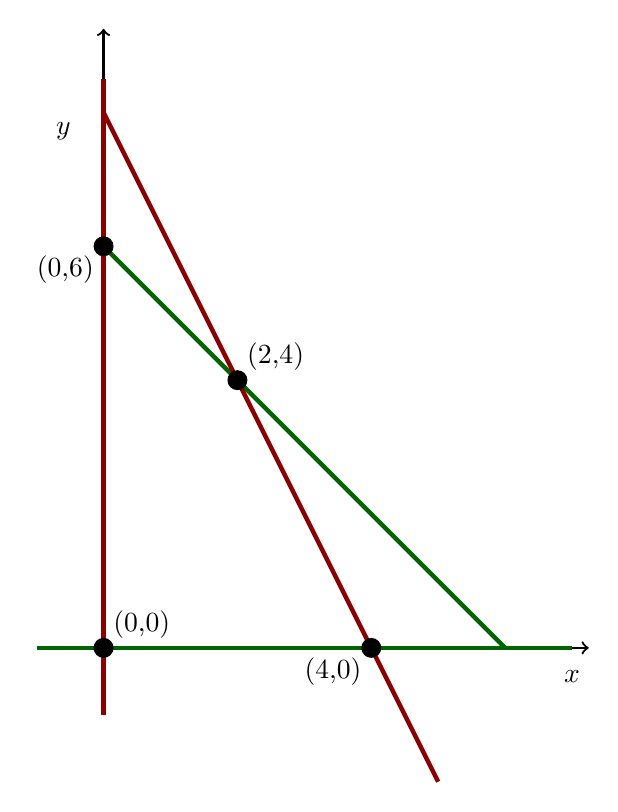
\begin{tikzpicture}[scale=0.85]
        \draw[thick, ->] (-1, 0) -- (7.25, 0);
        \draw[thick, ->] (0, -1) -- (0, 9.25);
        \node[overlay, below] at (7, -0.2) {$x$};
        \node[overlay, below] at (-0.6, 8) {$y$};   
        \draw[ultra thick,DarkGreen, -] (-1, 0) -- (7, 0);        
        \draw[ultra thick,DarkGreen, -] (0,6) -- (6, 0);   
        \draw[ultra thick,DarkRed, -] (0, 8) -- (5, -2);        
        \draw[ultra thick,DarkRed, -] (0, -1) -- (0, 8.5);      
        \filldraw[black] (0,0) circle (4pt) node[anchor=south west]{(0,0)};
        \filldraw[black] (0,6) circle (4pt) node[anchor=north east]{(0,6)};
        \filldraw[black] (2,4) circle (4pt) node[anchor=south west]{(2,4)};
        \filldraw[black] (4,0) circle (4pt) node[anchor=north east]{(4,0)};
        \end{tikzpicture}
        \end{center}            
        } 
        \else 
        \begin{center}
        \begin{tikzpicture}[scale=0.55]
        \draw[very thick, ->] (-6, 0) -- (6.25, 0);
        \draw[very thick, ->] (0, -6) -- (0, 6.25);
        \node[overlay, below] at (6, -0.2) {$x$};
        \node[overlay, below] at (-0.6, 6) {$y$};        
        \end{tikzpicture}
        \end{center}    
    \fi
    \end{parts}
\fi 





\ifnum \Version=2
    \question[6] Consider the non-linear system below.  
    \begin{align*}
        \dxdt &= (x-1)(y-5) , \qquad \dydt = y-x^2-1
    \end{align*}
    \begin{parts}
        \part Determine the locations of the critical points. 
        \ifnum \Solutions=1 {\color{DarkBlue} \\[12pt] 
        For a point to be a critical point, we need $x' = y' = 0$. If $x'$ is zero, then either $x=1$ or $y=5$. 
        \begin{itemize}
            \item When $x=1$, for $y'=0$ we need 
            \begin{align}
                y'&=0 = y - x^2 - 1 \quad \Rightarrow \quad y = 1^2+1 = 2
            \end{align}
            There is a critical point at $(1,2)$. 
            \item When $y=5$, for $y'=0$ we need 
            \begin{align}
                y'&=0 = y - x^2 - 1 \quad \Rightarrow \quad x^2 = 5 - 1 \quad \Rightarrow \quad x = \pm 2
            \end{align}
            There are critical points at $(\pm 2, 5)$.             
        \end{itemize}
            } 
        \else 
        \vfill
        \fi
        \part Sketch the nullclines of the system on the axes below. Clearly indicate the critical points that you found in part (a). 
        \ifnum \Solutions=1 {\color{DarkBlue} \\[12pt] 
        The curves are shown below. The green lines are the x nullclines, and the red curve is the y nullcline. There are exactly three critical points. 
            \begin{center}
            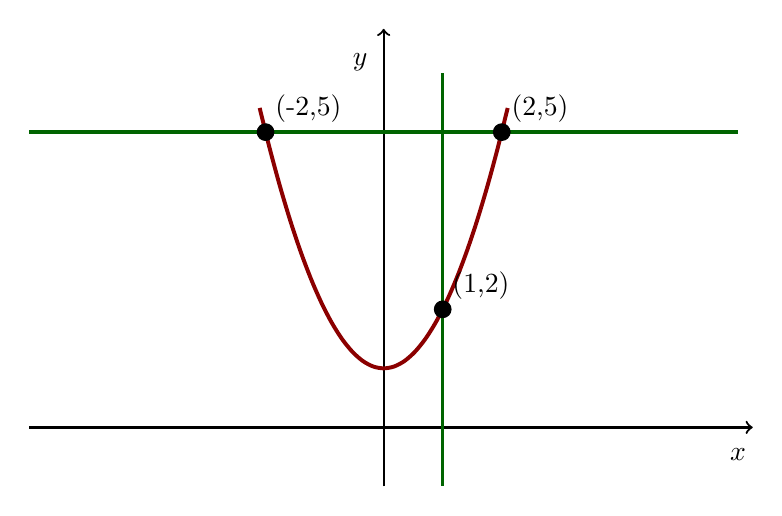
\begin{tikzpicture}[scale=0.75]
            \draw[thick, ->] (-6, 0) -- (6.25, 0);
            \draw[thick, ->] (0, -1) -- (0, 6.75);
            \node[overlay, below] at (6, -0.2) {$x$};
            \node[overlay, below] at (-0.4, 6.5) {$y$};   
            \draw[very thick,DarkGreen, -] (1, 6) -- (1, -1);        
            \draw[very thick,DarkGreen, -] (-6, 5) -- (6, 5);   
            \draw[DarkRed, line width = 0.50mm]   plot[smooth,domain=-2.1:2.1] (\x, {\x*\x+1});
            \filldraw[black] (2,5) circle (4pt) node[anchor=south west]{(2,5)};
            \filldraw[black] (-2,5) circle (4pt) node[anchor=south west]{(-2,5)};
            \filldraw[black] (1,2) circle (4pt) node[anchor=south west]{(1,2)};
            \end{tikzpicture}
            \end{center}               
        } 
        \else 
        \begin{center}
        \begin{tikzpicture}[scale=0.55]
        \draw[very thick, ->] (-6, 0) -- (6.25, 0);
        \draw[very thick, ->] (0, -6) -- (0, 6.25);
        \node[overlay, below] at (6, -0.2) {$x$};
        \node[overlay, below] at (-0.6, 6) {$y$};        
        \end{tikzpicture}
        \end{center}    
    \fi
    \end{parts}
\fi 




\ifnum \Version=3
    \question[6] Consider the non-linear system below.  
    \begin{align*}
        \dxdt &= (x-1)(y-2) , \qquad \dydt = y^2-x
    \end{align*}
    \begin{parts}
        \part Determine the locations of the critical points. 
        \ifnum \Solutions=1 {\color{DarkBlue} \\[12pt] 
        For a point to be a critical point, we need $x' = y' = 0$. If $x'$ is zero, then either $x=1$ or $y=2$. 
        \begin{itemize}
            \item When $x=1$, for $y'=0$ we need 
            \begin{align}
                y'&=0 = y^2 - x \quad \Rightarrow \quad y = \pm 1
            \end{align}
            There are critical points at $(1,\pm 1)$. 
            \item When $y=2$, for $y'=0$ we need 
            \begin{align}
                y'&=0 = y^2 - x  \quad \Rightarrow \quad x = 4 
            \end{align}
            There is a critical point at $(4, 2)$.             
        \end{itemize}
            } 
        \else 
        \vfill
        \fi
        \part Sketch the nullclines of the system on the axes below. Clearly indicate the critical points that you found in part (a). 
        \ifnum \Solutions=1 {\color{DarkBlue} \\[12pt] 
        The curves are shown below. The green lines are the x nullclines, and the red curve is the y nullcline. There are exactly three critical points. 
            \begin{center}
            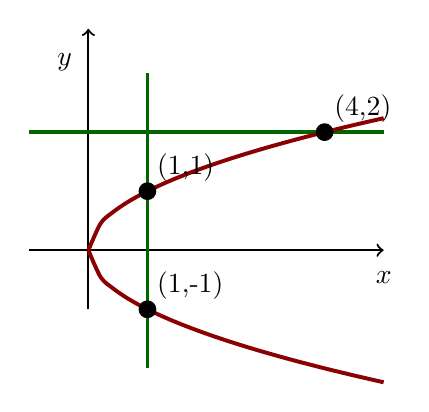
\begin{tikzpicture}[scale=0.75]
            \draw[thick, ->] (-1, 0) -- (5, 0);
            \draw[thick, ->] (0, -1) -- (0, 3.75);
            \node[overlay, below] at (5, -0.2) {$x$};
            \node[overlay, below] at (-0.4, 3.5) {$y$};   
            \draw[very thick,DarkGreen, -] (1, 3) -- (1, -2);        
            \draw[very thick,DarkGreen, -] (-1, 2) -- (5, 2);   
            \draw[DarkRed, line width = 0.50mm]   plot[smooth,domain=0:5] (\x, {\x^(1/2))} );
            \draw[DarkRed, line width = 0.50mm]   plot[smooth,domain=0:5] (\x, {-\x^(1/2))} );
            \filldraw[black] (4,2) circle (4pt) node[anchor=south west]{(4,2)};
            \filldraw[black] (1,1) circle (4pt) node[anchor=south west]{(1,1)};
            \filldraw[black] (1,-1) circle (4pt) node[anchor=south west]{(1,-1)};
            \end{tikzpicture}
            \end{center}               
        } 
        \else 
        \begin{center}
        \begin{tikzpicture}[scale=0.55]
        \draw[very thick, ->] (-6, 0) -- (6.25, 0);
        \draw[very thick, ->] (0, -6) -- (0, 6.25);
        \node[overlay, below] at (6, -0.2) {$x$};
        \node[overlay, below] at (-0.6, 6) {$y$};        
        \end{tikzpicture}
        \end{center}    
    \fi
    \end{parts}
\fi 


\ifnum \Version=6
    \question[4] Consider the non-linear system below.  
    \begin{align*}
        \dxdt &= (x-2)(y-1) , \qquad \dydt = 2y^2-x
    \end{align*}
    \begin{parts}
        \part Determine the locations of the critical points. 
        \ifnum \Solutions=1 {\color{DarkBlue} \\[12pt] 
        For a point to be a critical point, we need $x' = y' = 0$. If $x'$ is zero, then either $x=2$ or $y=1$. 
        \begin{itemize}
            \item When $x=2$, for $y'=0$ we need 
            \begin{align}
                y'&=0 = 2y^2 - x \quad \Rightarrow \quad y = \pm 1
            \end{align}
            There are critical points at $(2,\pm 1)$. 
            \item When $y=1$, for $y'=0$ we need 
            \begin{align}
                y'&=0 = 2y^2 - x  \quad \Rightarrow \quad x = 2
            \end{align}
            There is a critical point at $(2,1)$, which we already had.          
        \end{itemize}
            } 
        \else 
        \vfill
        \fi
        \part Sketch the nullclines of the system on the axes below. Clearly indicate the critical points that you found in part (a). 
        \ifnum \Solutions=1 {\color{DarkBlue} \\[12pt] 
        The curves are shown below. The green lines are the x nullclines, and the red curve is the y nullcline. There are exactly three critical points. 
            \begin{center}
            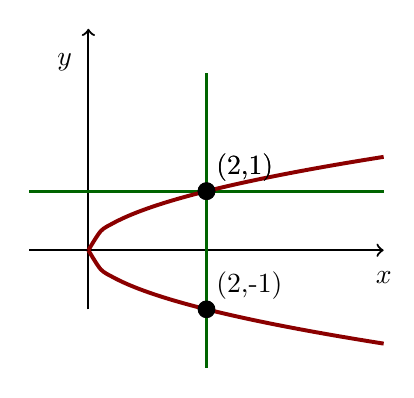
\begin{tikzpicture}[scale=0.75]
            \draw[thick, ->] (-1, 0) -- (5, 0);
            \draw[thick, ->] (0, -1) -- (0, 3.75);
            \node[overlay, below] at (5, -0.2) {$x$};
            \node[overlay, below] at (-0.4, 3.5) {$y$};   
            \draw[very thick,DarkGreen, -] (2, 3) -- (2, -2);        
            \draw[very thick,DarkGreen, -] (-1, 1) -- (5, 1);   
            \draw[DarkRed, line width = 0.50mm]   plot[smooth,domain=0:5] (\x, {(\x/2)^(1/2))} );
            \draw[DarkRed, line width = 0.50mm]   plot[smooth,domain=0:5] (\x, {-(\x/2)^(1/2))} );
            \filldraw[black] (2,1) circle (4pt) node[anchor=south west]{(2,1)};
            \filldraw[black] (2,1) circle (4pt) node[anchor=south west]{(2,1)};
            \filldraw[black] (2,-1) circle (4pt) node[anchor=south west]{(2,-1)};
            \end{tikzpicture}
            \end{center}               
        } 
        \else 
        \begin{center}
        \begin{tikzpicture}[scale=0.55]
        \draw[very thick, ->] (-6, 0) -- (6.25, 0);
        \draw[very thick, ->] (0, -6) -- (0, 6.25);
        \node[overlay, below] at (6, -0.2) {$x$};
        \node[overlay, below] at (-0.6, 6) {$y$};        
        \end{tikzpicture}
        \end{center}    
    \fi
    \end{parts}
\fi 


\ifnum \Version=7
    \question[4] Consider the non-linear system below.  
    \begin{align*}
        \dxdt &= (x-1)(y-5) , \qquad \dydt = y-x^2-1
    \end{align*}
    \begin{parts}
        \part Determine the locations of the critical points. 
        \ifnum \Solutions=1 {\color{DarkBlue} \\[12pt] 
        For a point to be a critical point, we need $x' = y' = 0$. If $x'$ is zero, then either $x=1$ or $y=5$. 
        \begin{itemize}
            \item When $x=1$, for $y'=0$ we need 
            \begin{align}
                y'&=0 = y - x^2 - 1 \quad \Rightarrow \quad y = 1^2+1 = 2
            \end{align}
            There is a critical point at $(1,2)$. 
            \item When $y=5$, for $y'=0$ we need 
            \begin{align}
                y'&=0 = y - x^2 - 1 \quad \Rightarrow \quad x^2 = 5 - 1 \quad \Rightarrow \quad x = \pm 2
            \end{align}
            There are critical points at $(\pm 2, 5)$.             
        \end{itemize}
            } 
        \else 
        \vfill
        \fi
        \part Sketch the nullclines of the system on the axes below. Clearly indicate the critical points that you found in part (a). 
        \ifnum \Solutions=1 {\color{DarkBlue} \\[12pt] 
        The curves are shown below. The green lines are the x nullclines, and the red curve is the y nullcline. There are exactly three critical points. 
            \begin{center}
            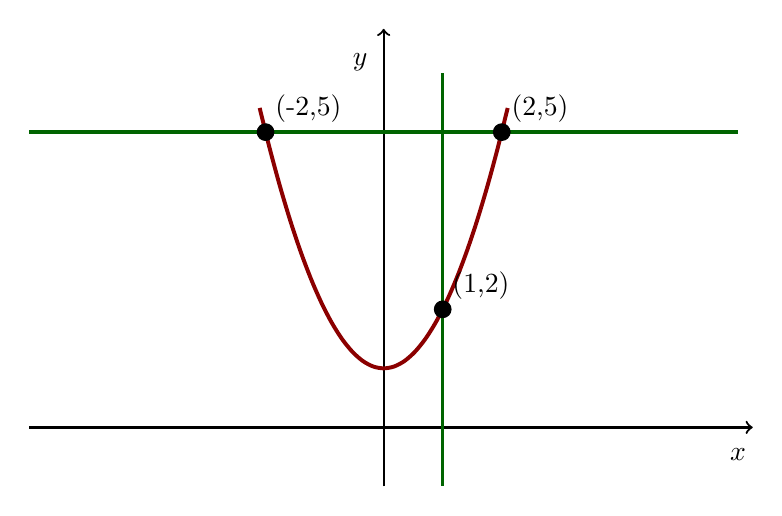
\begin{tikzpicture}[scale=0.75]
            \draw[thick, ->] (-6, 0) -- (6.25, 0);
            \draw[thick, ->] (0, -1) -- (0, 6.75);
            \node[overlay, below] at (6, -0.2) {$x$};
            \node[overlay, below] at (-0.4, 6.5) {$y$};   
            \draw[very thick,DarkGreen, -] (1, 6) -- (1, -1);        
            \draw[very thick,DarkGreen, -] (-6, 5) -- (6, 5);   
            \draw[DarkRed, line width = 0.50mm]   plot[smooth,domain=-2.1:2.1] (\x, {\x*\x+1});
            \filldraw[black] (2,5) circle (4pt) node[anchor=south west]{(2,5)};
            \filldraw[black] (-2,5) circle (4pt) node[anchor=south west]{(-2,5)};
            \filldraw[black] (1,2) circle (4pt) node[anchor=south west]{(1,2)};
            \end{tikzpicture}
            \end{center}               
        } 
        \else 
        \begin{center}
        \begin{tikzpicture}[scale=0.55]
        \draw[very thick, ->] (-6, 0) -- (6.25, 0);
        \draw[very thick, ->] (0, -6) -- (0, 6.25);
        \node[overlay, below] at (6, -0.2) {$x$};
        \node[overlay, below] at (-0.6, 6) {$y$};        
        \end{tikzpicture}
        \end{center}    
    \fi
    \end{parts}
\fi 

        \ifnum \Solutions=0
\newpage 
\fi
\ifnum \Version=1
\question[5] Consider the non-linear system below.  
\begin{align*}
    \dxdt &= x^2+y-2x-12 , \qquad \dydt = y-x-6
\end{align*}
The critical points are located at $(-2,4)$ and $(3,9)$. 
\begin{parts}
    \part Compute the Jacobian matrix, $J$, for the approximating linear system. 
    \ifnum \Solutions=1 {\color{DarkBlue}
        \begin{align}
            F &= x'\\
            G &= y' \\
            J &= \begin{pmatrix} F_x&F_y\\ G_x & G_y\end{pmatrix} = \begin{pmatrix} 2x-2&1\\-1&1\end{pmatrix}
        \end{align}
        } 
    \else 
    \vfill
    \fi        
    \part Use eigenvalues to classify the critical point at $(-2,4)$ according to stability (stable, unstable, asymptotically stable) and type (saddle, proper node, etc).
    \ifnum \Solutions=1 {\color{DarkBlue} \\[12pt] 
        At $(-2,4)$, $J = \begin{pmatrix} -6&1\\-1&1\end{pmatrix}$. The eigenvalues are the roots of \begin{align}
            (-6-\lambda)(1-\lambda)+1 = \lambda^2 +5\lambda - 5
        \end{align}
        Thus 
        \begin{align}
            \lambda = -\frac52 \pm \frac12 \sqrt{25-4\cdot(-5)} = -\frac52 \pm \frac{\sqrt{45}}{2}
        \end{align}
        $\lambda \in \mathbb R$, and the eigenvalues have opposite signs. The critical point is an unstable saddle. 
        } 
    \else 
    \vfill
    \fi
    \part Use eigenvalues to classify the critical point at $(3,9)$ according to stability (stable, unstable, asymptotically stable) and type (saddle, proper node, etc).
    \ifnum \Solutions=1 {\color{DarkBlue} \\[12pt] 
        At $(3,9)$, $J = \begin{pmatrix} 4&1\\-1&1\end{pmatrix}$. The eigenvalues are the roots of \begin{align}
            (4-\lambda)(1-\lambda)+1 = \lambda^2 - 5\lambda +5 
        \end{align}
        Thus 
        \begin{align}
            \lambda = \frac52 \pm \frac12 \sqrt{25-4\cdot(5)} = \frac52 \pm \frac{\sqrt{5}}{2}
        \end{align}
        $\lambda \in \mathbb R$, and the eigenvalues both positive. The critical point is an unstable node. 
    } 
    \else 
    \vfill
\fi
\end{parts}
\fi



\ifnum \Version=2
\question[6] Consider the non-linear system below.  
\begin{align*}
    \dxdt &= x(1-x-y) , \qquad \dydt = y(2-x-y)
\end{align*}
The critical points are located at $(0,0)$, $(0,2)$, and $(1,0)$. 
\begin{parts}
    \part Compute the Jacobian matrix, $J$, for the approximating linear system. 
    \ifnum \Solutions=1 {\color{DarkBlue} \\
    Set $ F = x'$ and $G = y'$. Then
        \begin{align}
            F_x &= 1 - 2x -y\\
            F_y &= -x \\
            G_x &= 2-x-2y \\
            G_y &= -y \\
            J &= \begin{pmatrix} F_x&F_y\\ G_x & G_y\end{pmatrix} = \begin{pmatrix} -1-x-2y & -x\\-y&2-x-2y \end{pmatrix}
        \end{align}
        } 
    \else 
    \vfill
    \fi        
    \part Use eigenvalues to classify the critical point at $(0,0)$ according to stability (stable, unstable, asymptotically stable) and type (saddle, proper node, etc).
    \ifnum \Solutions=1 {\color{DarkBlue} \\[12pt] 
        At $(0,0)$, $J = \begin{pmatrix} 1&0\\0&2\end{pmatrix}$. The eigenvalues are $\lambda = 1,2$. \\ Thus the critical point is an \textbf{unstable node}. 
        } 
    \else 
    \vfill
    \fi
    \part Use eigenvalues to classify the critical point at $(0,2)$ according to stability (stable, unstable, asymptotically stable) and type (saddle, proper node, etc).
    \ifnum \Solutions=1 {\color{DarkBlue} \\[12pt] 
        At $(0,2)$, $J = \begin{pmatrix} -1&0\\-2&-4\end{pmatrix}$. The eigenvalues are $\lambda = -1,-4$. \\Thus the critical point is a \textbf{stable node}. 
        } 
    \else 
    \vfill
    \fi
    \part Use eigenvalues to classify the critical point at $(1,0)$ according to stability (stable, unstable, asymptotically stable) and type (saddle, proper node, etc).
    \ifnum \Solutions=1 {\color{DarkBlue} \\[12pt] 
        At $(1,0)$, $J = \begin{pmatrix} -1&-1\\0&1\end{pmatrix}$. The eigenvalues are $\lambda = \pm 1$. \\ Thus the critical point is an \textbf{unstable saddle}. 
        } 
    \else 
    \vfill
    \fi    
\end{parts}
\fi










\ifnum \Version>5
\question[6] Consider the non-linear system below.  
\begin{align*}
    \dxdt &= x(4-x-y) , \qquad \dydt = y(6-2x-y)
\end{align*}
\begin{parts}
    \part Compute the Jacobian matrix, $J$, for the approximating linear system. 
    \ifnum \Solutions=1 {\color{DarkBlue} \\
    Set $ F = x'$ and $G = y'$. Then
        \begin{align}
            F &= 4x - x^2 - xy \\
            G &= 6y -2xy - y^2 \\
            J &= \begin{pmatrix} F_x&F_y\\ G_x & G_y\end{pmatrix} 
            = \begin{pmatrix} 4-2x-y & -x\\-2y& 6-2x-2y \end{pmatrix}
        \end{align}
        } 
    \else 
    \vfill
    \fi        
    \part Use eigenvalues to classify the critical point at $(0,6)$ according to stability (stable, unstable, asymptotically stable) and type (saddle, proper node, etc).
    \ifnum \Solutions=1 {\color{DarkBlue} \\[12pt] 
        At $(0,0)$, $J = \begin{pmatrix} -2&0\\-12&-6\end{pmatrix}$. The eigenvalues are $\lambda = -2, -6$. The CP is a \textbf{stable node}. 
        } 
    \else 
    \vfill
    \fi
    \part Use eigenvalues to classify the critical point at $(2,2)$ according to stability (stable, unstable, asymptotically stable) and type (saddle, proper node, etc).
    \ifnum \Solutions=1 {\color{DarkBlue} \\[12pt] 
        At $(0,2)$, $J = \begin{pmatrix} -2&-2\\-4&-2\end{pmatrix}$. Eigenvalues:
        \begin{align}
            0 &= (\lambda + 2)^2 - 8 = \lambda^2 + 4\lambda -4  \\
            \lambda &= -2 \pm \frac12 \sqrt{16 + 16} = -2 \pm 2\sqrt 2
        \end{align}\\Thus the critical point is an \textbf{unstable saddle}. 
        } 
    \else 
    \vfill
    \fi
\end{parts}
\fi

  
        \ifnum \Solutions=0
\newpage 
\fi

\ifnum \Version=1    
\question[2] 
Compute the Laplace transform of the function below. Do not leave your answer in terms of an integral. Please show your work. 
$$y(t) = \begin{cases} 0, \quad 0 \le t < 1 \\ t-2, \quad 1 \le t < 3 \\ 0, \quad 3 \le t < \infty\end{cases}$$
\ifnum \Solutions=1 {\color{DarkBlue} \\[12pt] 
There are a few different ways to solve this. Any of the approaches below are sufficient. 
\subsection*{Method 1: Direct Integration }
Direct integration requires integration by parts, but using the definition of the Laplace Transform:
    \begin{align}
        \int_0^{\infty} e^{-st} y(t) \, dt 
        &= \int_1^{3} e^{-st} \, (t-2) \, dt \\
        &= \int_1^{3} te^{-st}  \, dt - 2 \int_1^{3} e^{-st}  \, dt \\
        &=  \left. t\cdot \frac{-1}{s}e^{-st} \right|_1^3
        - \int_1^{3} \frac{-1}{s}e^{-st} \, dt 
        -2 \left( \left. \frac{-1}{s}e^{-st}\right|_{t=1}^{t=3}\right) \\
        &=  \frac{-1}{s}\left( 3e^{-3s} - e^{-s} \right)  
        + \frac{1}{s} \int_1^{3} e^{-st} \, dt 
        + \frac{2}{s} \left(  e^{-3s} - e^{-s} \right) \\
        &=  \frac{-1}{s}\left( 3e^{-3s} - e^{-s} \right)  
        + \frac{1}{s} \left( \left. \frac{-1}{s}e^{-st}\right|_{t=1}^{t=3}\right) \, dt 
        + \frac{2}{s} \left(  e^{-3s} - e^{-s} \right) \\     
        &=  \frac{-1}{s}\left( 3e^{-3s} - e^{-s} \right)  
        - \frac{1}{s^2} \left(  e^{-3s} - e^{-s} \right) 
        + \frac{2}{s} \left(  e^{-3s} - e^{-s} \right) \\      
        &= - \frac{1}{s^2} \left(  e^{-3s} - e^{-s} \right) 
        - \frac{ e^{-3s}}{s}   - \frac{e^{-s}}{s}  \\   
        &= \frac{e^{-s}}{s^2} - \frac{e^{-3s}}{s^2} 
        - \frac{ e^{-3s}}{s}   - \frac{e^{-s}}{s}           
    \end{align}
    \subsection*{Method 2: Step Functions}
    We could also use the table of transforms, specifically the transform of the step function $u_c(t)$ and its product with another function. 
    \begin{align}
        y(t) &= 0u_{0,1} + (t-2)u_{1,3} + 0u_{3} 
        =(t-2)(u_1-u_3) 
        = tu_1-tu_3 - 2u_1 + 2 u_3 
    \end{align}   
    At this point we can either take the transform and use the derivative theorem (in the table) to work out the transform of $tu_1$ and $tu_3$, or we can use the following trick:
    \begin{align}
        y(t) &= tu_1-tu_3 - 2u_1 + 2 u_3 \\
        &= (t+1-1)u_1-(t+3-3)u_3 - 2u_1 + 2 u_3 \\
        &= (t-1)u_1 + u_1 -(t-3)u_3 - 3u_3 - 2u_1 + 2 u_3 \\
        &= (t-1)u_1 -(t-3)u_3 - u_1 - u_3 
    \end{align}
    Using the table of transforms the Laplace transform is
    \begin{align}
        Y(s) = \frac{e^{-s}}{s^2} - \frac{e^{-3s}}{s^2} - \frac{e^{-s}}{s} - \frac{e^{-3s}}{s}
    \end{align}
} 
\else 
    \vfill
    \begin{center}
        \textit{This remainder of this page can be used for scratch work. }
    \end{center}
    \vfill
\fi
\fi


\ifnum \Version=5
\question[2] 
Compute the Laplace transform of the function below. Do not leave your answer in terms of an integral. Please show your work. 
$$y(t) = \begin{cases} 0, \quad 0 \le t < 1 \\ 4, \quad 1 \le t < 3 \\ 0, \quad 3 \le t < \infty\end{cases}$$
\ifnum \Solutions=1 {\color{DarkBlue} \\[12pt] 
There are a few different ways to solve this. Any of the approaches below are sufficient. 
\subsection*{Method 1: Direct Integration }
Direct integration uses the definition of the Laplace Transform:
    \begin{align}
        \int_0^{\infty} e^{-st} y(t) \, dt 
        = \int_1^{3} e^{-st} \, 4 \, dt 
        &= 4\int_1^{3} e^{-st}  \, dt  \\         
        &= 4\left.\frac{-1}{s} e^{-st} \right|_1^3  \\         
        &= \frac{-4}{s} \left(e^{-3s}  - e^{-s} \right)     
    \end{align}
    \subsection*{Method 2: Step Functions}
    We could also use the table of transforms, specifically the transform of the step function $u_c(t)$ and its product with another function. 
    \begin{align}
        y(t) &= 0u_{0,1} + 4u_{1,3} + 0u_{3} 
        =4(u_1-u_3) 
        = 4u_1 - 4 u_3 
    \end{align}   
    Using the table of transforms the Laplace transform is
    \begin{align}
        Y(s) = 4 \frac{e^{-s}}{s} - 4\frac{e^{-3s}}{s}
    \end{align}
    \newpage
} 
\else 
    \vfill
    \begin{center}
        \textit{This remainder of this page can be used for scratch work. }
    \end{center}
    \vfill
\fi
\fi







\ifnum \Version=6
\question[3] 
The function $f(t)$ is periodic, has period $4$, and 
        $$f(t) = \begin{cases} e^{-3t}, \quad 0 \le t < 2 \\ 0, \quad 2 \le t < 4 \end{cases}$$
        Compute the Laplace transform of $f(t)$. Do not leave your answer in terms of an integral. Please show your work. 

\ifnum \Solutions=1 {\color{DarkBlue} 
    We use the formula for a periodic function with $T=4$. 
    
        With $T=4$,
        
        \begin{align}
            \mathcal{L}\{f(t)\} &=  \frac{\int_{0}^{T} e^{-st} f(t) dt}{1 - e^{-Ts}} \\
            &= \frac{1}{1 - e^{-4s}} \left( \int_{0}^{2} e^{-st} e^{-3t} dt + \int_2^4 0 \, dt \right)\\
            &= \frac{1}{1 - e^{-4s}} \cdot \frac{1}{-s-3} \left. e^{(-s-3)t}\right|_0^2 \\
            &= -\frac{1}{1 - e^{-4s}} \cdot \frac{1}{s+3} \left( e^{-2(s+3)} - 1 \right)
        \end{align}
        \newpage
} 
\else 
    \newpage
    \begin{center}
        \textit{This remainder of this page can be used for scratch work. }
    \end{center}
    \vfill
\fi
\fi



\ifnum \Version=7
\question[3] 
The function $f(t)$ is periodic, has period $4$, and 
        $$f(t) = \begin{cases} e^{-2t}, \quad 0 \le t < 3 \\ 0, \quad 3 \le t < 4 \end{cases}$$
        Compute the Laplace transform of $f(t)$. Do not leave your answer in terms of an integral. Please show your work. 

\ifnum \Solutions=1 {\color{DarkBlue} 
    We use the formula for a periodic function with $T=4$. 
    
        With $T=4$,
        
        \begin{align}
            \mathcal{L}\{f(t)\} &=  \frac{\int_{0}^{T} e^{-st} f(t) dt}{1 - e^{-Ts}} \\
            &= \frac{1}{1 - e^{-4s}} \left( \int_{0}^{3} e^{-st} e^{-2t} dt + \int_3^4 0 \, dt \right)\\
            &= \frac{1}{1 - e^{-4s}} \cdot \frac{1}{-s-2} \left. e^{(-s-2)t}\right|_0^3 \\
            &= -\frac{1}{1 - e^{-4s}} \cdot \frac{1}{s+2} \left( e^{-3(s+2)} - 1 \right)
        \end{align}
} 
\else 
    \newpage
    \begin{center}
        \textit{This remainder of this page can be used for scratch work. }
    \end{center}
    \vfill
\fi
\fi




    \fi 
\end{questions}